\documentclass[11pt]{article}

\usepackage[utf8]{inputenc}
\usepackage[T1]{fontenc}
\usepackage{graphicx}
\usepackage{amsmath}
\usepackage{amssymb}
\usepackage{booktabs}
\usepackage{longtable}
\usepackage{array}
\usepackage{siunitx}
\usepackage[margin=1in]{geometry}
\usepackage{natbib}
\usepackage{caption}
\usepackage{lineno}
\usepackage{tikz}
\usetikzlibrary{arrows.meta,backgrounds,positioning,fit,shapes.geometric}
\usepackage[colorlinks=true,linkcolor=blue,citecolor=blue,urlcolor=blue]{hyperref}

\graphicspath{{../figures/}}

\newcolumntype{L}[1]{>{\raggedright\arraybackslash}p{#1}}
\newcolumntype{C}[1]{>{\centering\arraybackslash}p{#1}}
\setlength{\tabcolsep}{4pt}

\title{Carbon-plate insole use and self-reported injury prevalence among\\
Italian competitive athletics athletes: a cross-sectional, Bayesian\\
multilevel analysis of a two-phase recruited cohort}
\author{Anonymized Author 1 \and Anonymized Author 2}
\date{}

\begin{document}
\linenumbers
\modulolinenumbers[1]

\maketitle
\label{sec:title}

\begin{abstract}
\label{sec:abstract}
\textbf{Objective:} To describe carbon-plate insole use during preparation and competition among competitive Italian athletics athletes, estimate its cross-sectional, period-matched association with self-reported current-season injury, and examine whether that association was better characterized by relative carbon share or absolute carbon-use frequency.

\textbf{Design:} Cross-sectional survey with two-phase (voluntary, then targeted-recall) recruitment, poststratified to national age--sex population strata; reported in line with STROBE and the STROBE Sports Injury and Illness Surveillance (STROBE-SIIS) extension.

\textbf{Participants:} FIDAL-affiliated athletics athletes (Under 20, Under 23, Senior categories) recruited nationally in 2026. Of 355 eligible, complete respondents, 352 (704 athlete-period records) formed the balanced analysis cohort.

\textbf{Exposure:} Carbon share (the proportion of reported weekly training-type frequency delivered in carbon-plated spikes) and absolute carbon-frequency score (the summed carbon-frequency items) across five training domains, calculated separately for preparation and competition.

\textbf{Outcome:} Self-reported injury occurring in the preparation period and/or the competition period of the current season.

\textbf{Statistical methods:} Bayesian multilevel logistic models used period-specific intercepts, an athlete-level random intercept, and adjustment for demographic, anthropometric, period-matched training-frequency, and discipline covariates. The primary model represented carbon share among users with a continuous, data-driven curve fitted by a Hilbert-space Gaussian process, letting the amount of curvature in the dose--response relationship be estimated rather than fixed in advance. Two matched linear models then evaluated competing relative-use (carbon share) and absolute-use (carbon-frequency score) hypotheses on a common among-user standard-deviation scale. Estimands included adjusted prevalence contrasts and conditional absolute-risk differences for a fixed reference profile.

\textbf{Results:} Carbon-plated spikes accounted for a mean 35.7\% of reported preparation training and 47.7\% of reported competition training. Adoption showed no clear association with injury in either period. The primary curve showed adjusted competition-period injury prevalence climbing steadily with carbon share; moving from the 25th to 75th percentile of competition-period carbon share was associated with a 13.2-percentage-point higher adjusted injury prevalence (95\% CrI $-0.2$ to 29.1; $P_{\mathrm{dir}}=96.9\%$), the strongest of the four primary contrasts and the only one clearing the pre-specified practical-relevance threshold. In the matched linear comparison, a one-standard-deviation increase meant 24.1 percentage points of carbon share (37.3\% to 61.4\%) or 3.36 units of the summed ordinal carbon-frequency score (2.83 to 6.19). Among competition users, these increments corresponded to risk differences of 7.9 points for share (95\% CrI 1.4 to 14.4; $P_{\mathrm{dir}}=99.0\%$) and 8.3 points for absolute score (95\% CrI 1.6 to 15.9; $P_{\mathrm{dir}}=99.2\%$); preparation-period estimates were 3.6 points (95\% CrI $-3.9$ to 11.2; $P_{\mathrm{dir}}=82.8\%$) and 1.5 points (95\% CrI $-6.9$ to 9.4; $P_{\mathrm{dir}}=63.2\%$), respectively.

\textbf{Conclusion:} Among competition users, greater reported carbon exposure was associated with higher adjusted injury prevalence whether expressed as relative share or absolute frequency score; these data did not identify one scale as the better explanation. Adoption and preparation-period exposure were not clearly associated with injury. The cross-sectional, retrospective design does not support causal interpretation.

\end{abstract}

\noindent\textbf{Keywords:} athletics; track and field; carbon-fiber plate; advanced footwear technology; injury surveillance; Bayesian multilevel model; STROBE-SIIS.

\section{Introduction}
\label{sec:introduction}
Athletics (track and field) carries a substantial burden of health problems at the competitive tiers of participation \citep{mckay2022tier}. A systematic review and meta-analysis of 216 studies in Olympic athletics disciplines reported a mean injured-athlete prevalence of 50.4\% (range 2.4\%--93.6\%) and a mean incidence of 135.6 injuries per 1000 registered athletes, with injury patterns differing markedly by discipline group, tissue type, and period of the season \citep{edouard2020injury}. Roughly half of injuries in youth athletics academies were reported in the winter preparation period \citep{martinezsilvan2021injury}, motivating separate description of preparation- and competition-period injury rather than a single season-level estimate.

How injury is registered materially changes the burden observed. Surveillance restricted to absence, complete sports cessation, or medical attention can under-ascertain overuse problems because athletes may continue training and competing despite symptoms and impaired function \citep{clarsen2013ostrc}. The Oslo Sports Trauma Research Center Questionnaire on Health Problems (OSTRC-H) therefore complements time-loss registration with direct athlete reports across four impact domains: sports participation, training volume, performance, and symptoms \citep{clarsen2014ostrch,clarsen2020ostrc}. These domains provide an athlete-reported measure of sport-specific health burden; they should not be interpreted as a generic quality-of-life scale.

Since 2020--2021, competitive athletics has undergone a rapid equipment transition with the introduction of ``advanced footwear technology'' (AFT) spikes: a rigid, longitudinally curved carbon-fiber plate embedded in a high-resilience foam midsole, first validated in road racing (Nike Vaporfly, Breaking2 project) and subsequently extended to track spikes for sprint and middle-distance events \citep{healey2022superspikes}. The stated biomechanical rationale is that plate-driven longitudinal bending stiffness reduces energy dissipation at the metatarsophalangeal joints and shifts the center of pressure anteriorly, increasing horizontal propulsive force \citep{willwacher2016stiffness}. Comparative analyses of world-leading sprint performance before and after the introduction of AFT spikes have documented step changes in top-100 performance lists coincident with the technology's diffusion \citep{mason2023superspikes}.

The same mechanical changes that plausibly improve performance also alter loading at the ankle and forefoot. A recent kinetic comparison of traditional and carbon-plated sprint spikes in elite sprinters found materially higher ankle joint contact force and higher peak plantarflexor muscle force in the carbon-plated condition, with pronounced inter-individual variability \citep{gerlach2025aft}. Case reports and narrative reviews have raised the possibility of increased Achilles tendon load and of altered forces at the navicular and cuneiform bones, both recognized high-risk sites for bone stress injury in runners \citep{tenforde2023bonestress}. Evidence on ground-reaction-force-mediated risk is mixed, and no consensus exists on whether increased longitudinal bending stiffness is protective, neutral, or hazardous once inter-individual differences in plantarflexor strength are taken into account \citep{willwacher2016stiffness,gerlach2025aft}.

Despite this plausible mechanistic pathway, direct epidemiological evidence on carbon-plate insole use and injury in competitive athletics is essentially absent: available data are limited to isolated case reports and small mechanistic cohorts, none of which were designed to estimate population-level injury associations \citep{tenforde2023bonestress,gerlach2025aft}. Established risk factors for running-related injury more broadly include age, body mass index, weekly training frequency, footwear, years of sporting experience, and prior injury \citep{taunton2003running}, all of which needed to be accounted for before any exposure--outcome association attributable to carbon-plate use could be considered informative.

This study was designed to close part of this gap by describing carbon-plate insole use among a national sample of Italian competitive athletics athletes and by estimating the cross-sectional, period-matched association between reported carbon share and self-reported injury during the preparation and competition periods of a single season. Consistent with the Injury Definitions Concept Framework and the athletics-specific consensus statement on injury and illness surveillance \citep{timpka2014consensus,timpka2015meta}, injury was defined broadly as a physical complaint or observable tissue damage attributable to the transfer of energy experienced by an athlete during training or competition participation in athletics, irrespective of whether medical attention was sought or of the consequences for participation \citep{bahr2020strobesiis}. The primary hypothesis, formulated a priori, was that greater reported carbon share would be associated with higher adjusted injury prevalence; a secondary, exploratory aim was to describe whether carbon-plate adoption and share differed by age group and sex, and whether the exposure--outcome association was stable under population reweighting and alternative dose--response specifications.


\section{Methods}
\label{sec:methods}
\subsection{Study design and reporting}
\label{sec:design}
This is a retrospective, cross-sectional survey study of competitive athletics athletes affiliated with the Federazione Italiana di Atletica Leggera (FIDAL). Reporting follows the STROBE statement and its athletics-relevant STROBE Sports Injury and Illness Surveillance (STROBE-SIIS) extension \citep{vonelm2007strobe,bahr2020strobesiis}; the completed checklist, with the manuscript line number supporting each item, is given in Appendix~\ref{sec:strobe-checklist}.

\subsection{Study registration}
\label{sec:registration}
This study was not registered in a public trial or study registry (for example, ClinicalTrials.gov or an equivalent observational-study registry). It was, however, prospectively specified through a complete study protocol, submitted in Italian and reviewed and approved by the Comitato Etico of the University of Turin (Section~\ref{sec:setting}) before survey deployment. The protocol specified the study population, the two-phase recruitment and poststratification strategy, the exposure and outcome definitions, and the primary hypothesis (Section~\ref{sec:introduction}) in advance of data collection and of any outcome analysis. This ethics-committee-reviewed protocol is the prospective record of the study design; it is not, however, a substitute for public registration, and the absence of the latter is noted as a limit on independent, external verification of pre-specification (Section~\ref{sec:discussion-limitations}).

\subsection{Setting and ethics}
\label{sec:setting}
Data collection used a structured, self-administered online survey covering demographic, anthropometric, training, footwear, and injury-history items for the current competitive season, separately for the preparation and competition periods. Study data were collected and managed using REDCap electronic data capture tools hosted at the Department of Clinical and Biological Sciences, University of Turin \citep{harris2009redcap,harris2019redcap}. REDCap (Research Electronic Data Capture) is a secure, web-based software platform designed to support data capture for research studies, providing (1) an intuitive interface for validated data capture, (2) audit trails for tracking data manipulation and export procedures, (3) automated export procedures for seamless data downloads to common statistical packages, and (4) procedures for data integration and interoperability with external sources.

The study was approved by the Comitato Etico of the University of Turin (protocol n. 0453001, approved 23 June 2026). Participation required electronic informed consent; no financial incentive was offered. Individual survey responses were stored under a study identifier disconnected from athlete names at the point of analysis; only aggregate, de-identified data and model outputs are reported here, in line with the data-privacy provisions of the Declaration of Helsinki.

\subsection{Participants and two-phase recruitment}
\label{sec:participants}
Eligible athletes were FIDAL-affiliated competitive athletes in the Under 20, Under 23, or Senior (\emph{assoluta}) categories, across seven athletics disciplines with adequate cell support in the sample (sprint, middle distance, long distance, hurdles, horizontal jumps, pole vault, combined events; four further disciplines had zero respondents and were dropped from discipline-level adjustment; Appendix Table~\ref{tab:discipline-support}).

Recruitment proceeded in two phases to reduce the risk that a purely voluntary sample would over-represent already engaged or higher-exposure athletes. In Phase 1, the survey was distributed openly through FIDAL-affiliated clubs and athlete networks; enrollment was entirely voluntary. National population totals by age category, sex, and discipline group were estimated from FIDAL competition-registry history (Appendix Table~\ref{tab:population-frame-history}). Study size was planned for precision of a population proportion rather than power for a specific exposure association. For each candidate sample size $n$, the worst-case count $x=\lfloor n/2\rfloor$ was combined with a Beta(1,1) prior, giving a Beta$(1+x,1+n-x)$ posterior; the smallest $n$ whose equal-tailed 95\% credible interval had half-width no greater than 0.06 was selected. This rule gave $n=264$ from the estimated eligible frame of 1328 athletes (19.9\%); targets were allocated proportionally across the 42 age-by-sex-by-discipline strata using largest-remainder rounding (Appendix Table~\ref{tab:sample-size}). The calculation established a minimum precision and population-coverage target, not representativeness by itself. After Phase 1 closed, strata that had not reached their target count were identified, and Phase 2 undertook targeted recall--direct outreach to athletes and clubs within under-represented age-by-sex-by-discipline strata--until every stratum met or approached its target or the recruitment window closed. Detailed recruitment-monitoring cells are retained privately to avoid disclosing small-cell participation patterns. This two-phase design does not produce a probability sample with known, non-zero, equal selection probabilities in every stratum; population coverage was supported by targeted recruitment, and residual over- and under-representation was corrected analytically (Section~\ref{sec:weighting}) rather than assumed away.

Of all survey respondents, 355 provided consent, met calculated eligibility, and completed the survey (\texttt{survey\_atleta\_it\_complete = 2}). One athlete was excluded for incomplete injury-timing data, and two further athletes were excluded because a period (preparation or competition) had a zero total eligible training-frequency score, precluding a carbon-share denominator. The final balanced analysis cohort comprised 352 athletes contributing 704 athlete-period records (one preparation and one competition record per athlete; Table~\ref{tab:sample-flow}).

\subsection{Exposure: carbon-plate insole use}
\label{sec:exposure}
For each period (preparation, competition) and each of five training domains--long endurance, middle endurance, lactate, maximum velocity, and technique--athletes reported an ordinal weekly training-type frequency (0, 1, 2, 3, 4, or 5-or-more sessions per week, with 5-or-more coded as 5) separately for sessions performed in carbon-plated spikes and sessions performed without them. \emph{Carbon share} for a given period was defined as
\[
\text{carbon share} = \frac{\sum \text{carbon-frequency items}}{\sum \text{carbon-frequency items} + \sum \text{non-carbon-frequency items}},
\]
summed across the five domains. The corresponding \emph{absolute carbon-frequency score} was the numerator alone, that is, the sum of the five carbon-frequency items. It is an ordinal frequency score rather than an exact count of unique sessions because responses were top-coded at five and a session could contribute to more than one reported training domain. Gym/strength conditioning (\emph{palestra}) has no carbon-eligible equivalent and was retained only as a non-carbon adjustment covariate, not in the carbon-share denominator. Carbon share is therefore a composition of reported ordinal training-type frequency, not a directly measured training-time proportion or shoe-wear duration; this distinction is carried through to the interpretation of all exposure estimands. Exposure was decomposed into two components: \emph{adoption} (any carbon use versus none, \texttt{carbon\_frequency\_sum > 0}) and, among users, continuous \emph{dose}, expressed primarily as carbon share and additionally as the absolute carbon-frequency score.

\subsection{Outcome: period-specific injury}
\label{sec:outcome}
The outcome was self-reported injury attributable to athletics training or competition participation during the current season, following the athletics-specific consensus definition \citep{bahr2020strobesiis,timpka2014consensus}: any physical complaint or observable tissue damage resulting from the transfer of energy experienced by an athlete during participation, regardless of medical attention sought or time-loss consequence. Athletes reported the number of current-season injuries (0, 1, or 2) and, for each, whether onset occurred in the preparation period, the competition period, or both (coded 1, 2, or 3 respectively). Preparation-period injury was defined as any reported injury coded 1 or 3; competition-period injury as any reported injury coded 2 or 3. Athletes could therefore contribute a positive outcome to one or both periods.

For each reported injury, athletes also selected the anatomical location (hip, groin, thigh, lower leg, ankle, foot, or head/upper limb/trunk; multi-select) and, only for injuries localized to the lower limb, the injury type (joint sprain, tendon rupture, ligament injury, muscle strain, bone stress injury or stress fracture, tendinopathy, plantar fasciopathy, or other; multi-select, adapted from consensus-recommended categories \citep{bahr2020strobesiis}). These location and type items were not used as covariates or outcomes in the primary Bayesian model; they are reported descriptively (Section~\ref{sec:results-pattern}) to characterize the injury pattern in this cohort, following STROBE-SIIS item SIIS17.1. Injury severity (time-loss duration) was also collected but is outside the scope of the present analysis.

Athletes reporting at least one current-season injury were also presented with four items adapted from the updated OSTRC-H2, covering the injury's impact on sports participation, training volume, sports performance, and symptoms \citep{clarsen2014ostrch,clarsen2020ostrc}. The four ordered responses were scored 0, 8, 17, and 25, then summed to an adapted OSTRC severity score from 0 (no reported impact) to 100 (maximum reported impact). Because these items were administered once retrospectively and only after a current-season injury was reported, the score is used solely as a descriptive athlete-reported impact measure; it is not a prospective weekly OSTRC prevalence or cumulative-burden estimate.

\subsection{Covariates}
\label{sec:covariates}
Adjustment covariates were age (years), competition sex, height (cm), body mass (kg), years of athletics experience, injury in either of the two preceding seasons (binary), period-matched total training-type-frequency scores for each of the five domains and for \emph{palestra}, and indicator variables for the seven discipline categories with non-zero support. These variables were selected a priori based on previously reported risk factors for running-related injury \citep{taunton2003running} and on the requirement, specified in the STROBE-SIIS extension, to account for how athletes were categorized by sport, discipline, and competitive level \citep{bahr2020strobesiis}. Continuous covariates were standardized (zero mean, unit variance) before model fitting.

\subsection{Statistical methods}
\label{sec:statistics}
All inference is Bayesian \citep{gelman2013bda}; no null-hypothesis-testing framework or $p$-values are reported. Results are summarized as posterior means, medians, standard deviations, and 95\% credible intervals (CrI, equal-tailed 2.5th--97.5th percentiles). Every reported interval for a signed association contrast is accompanied by its posterior probability of direction, $P_{\mathrm{dir}}=\max\{P(\Delta>0),P(\Delta<0)\}$ (with one replacing zero as the null for ratios): the posterior probability that the contrast lies on the same side of the null as its median estimate. This is a graded measure of directional certainty, not a $p$-value or a binary significance test, and it must be read together with the effect magnitude and CrI. $P_{\mathrm{dir}}$ is not reported for absolute prevalences, for which positivity is constrained by definition and therefore uninformative. We additionally report posterior probabilities that an association exceeds a pre-specified practically relevant threshold (5 percentage points for differences, a ratio of 1.10) or falls within a region of practical equivalence to no association ($\pm$2 percentage points; ratio 0.95--1.05). Models were fit in Stan \citep{carpenter2017stan} via its R interface.

The adapted OSTRC scores were summarized by mutually exclusive injury-period groups (preparation only, competition only, or both periods) using medians and interquartile ranges. As a descriptive effect-size aid, standardized mean differences (SMD) compared preparation-only and both-period groups with the competition-only group, calculated as the mean-score difference divided by the square root of the average of the two group variances. No injured-versus-uninjured OSTRC comparison was made because the items were not administered to uninjured athletes.

\subsubsection{Primary model}
\label{sec:primary-model}
Each athlete contributed one Bernoulli outcome per period. A shared athlete-level random intercept linked the two outcomes, following a cluster-specific logistic formulation for correlated binary data \citep{neuhaus1991correlated}. For athlete $i$ in period $p$,
\[
Y_{ip}\sim\operatorname{Bernoulli}(\pi_{ip}),
\qquad
\operatorname{logit}(\pi_{ip})=\alpha_p+c_{ip}+a_{ip}+\delta_i+u_i,
\qquad
u_i\sim\mathcal{N}(0,\sigma_u^2).
\]
Here $c_{ip}$ is the carbon-use contribution:
\[
c_{ip}=\begin{cases}
0, & \text{for a non-user},\\
\beta^{\text{any}}_p+f_p(\text{share}_{ip}), & \text{for a carbon user}.
\end{cases}
\]
The remaining terms have direct roles: $\alpha_p$ is the period-specific intercept, $a_{ip}$ combines the athlete-level and period-matched covariates of Section~\ref{sec:covariates}, $\delta_i$ is the partially pooled discipline contribution, and $u_i$ is the athlete random intercept. The function $f_p$ is a period-specific curve over carbon share among users, given a Hilbert-space approximate Gaussian-process (HSGP) prior with a Mat\'ern-5/2 kernel \citep{riutortmayol2023hsgp}, fitted with a common basis and centered at the pooled median user share (0.50):
\[
f_p(\text{share}_{ip}) = \sum_{m=1}^{40} \phi_m(\text{share}_{ip})\, b_{p,m},
\qquad
b_{p,m} \sim \mathcal N\!\left(0,\, S\!\left(\sqrt{\lambda_m};\, \alpha^{\text{gp}}_p, \rho^{\text{gp}}_p\right)\right),
\]
where $\phi_m$ and $\lambda_m$ are the eigenfunctions and eigenvalues of the Laplace operator on the centered, boundary-extended domain $[-0.75, 0.75]$ (a boundary factor of 1.5 times the largest centered observed user share), $S(\cdot)$ is the Mat\'ern-5/2 spectral density, and $\alpha^{\text{gp}}_p$ and $\rho^{\text{gp}}_p$ are period-specific marginal-standard-deviation and length-scale hyperparameters estimated from the data. This construction lets the posterior determine how much curvature the competition- and preparation-period dose--response relationships each support directly from the data, through $\alpha^{\text{gp}}_p$ and $\rho^{\text{gp}}_p$. 40 basis functions were confirmed sufficient by checking that the spectral density at the highest included frequency was negligible relative to the lowest across both hyperparameters' posterior distributions. Consequently, $\beta^{\text{any}}_p$ compares a median-share user with a non-user on the conditional log-odds scale, while $f_p$ describes dose among users. The athlete and discipline terms, and the HSGP basis coefficients $b_{p,m}$, were parameterized non-centered, with discipline coefficients partially pooled through a shared scale $\tau_{\text{disc}}$. Priors were regularizing and weakly informative on the standardized log-odds scale: $\alpha_p\sim\mathcal{N}(\operatorname{logit}(0.4),1.5^2)$, $\beta^{\text{any}}_p\sim\mathcal N(0,0.7^2)$, covariate coefficients $\mathcal{N}(0, 0.5^2)$, $\tau_{\text{disc}} \sim \text{Half-N}(0, 0.5^2)$, $\sigma_u \sim \text{Half-N}(0, 1^2)$, $\alpha^{\text{gp}}_p \sim \text{Half-N}(0, 0.7^2)$, and $\rho^{\text{gp}}_p \sim \text{Inv-Gamma}(2.94, 0.80)$, the last chosen so that its 1st and 99th prior percentiles fell at one-tenth and twice the observed centered-share range, discouraging length scales too short for the data to resolve while still permitting substantial curvature. A matched baseline model retained the identical outcome, covariate, discipline, and athlete-random-intercept structure but removed both carbon-use terms, providing a no-exposure comparator for predictive-validity assessment (Section~\ref{sec:validation}).

Figure~\ref{fig:primary-model-graph} summarizes the primary model's observed inputs, parameter hierarchy, and repeated athlete-period outcome structure.
\begin{figure}[htbp]
\centering
\resizebox{\textwidth}{!}{%
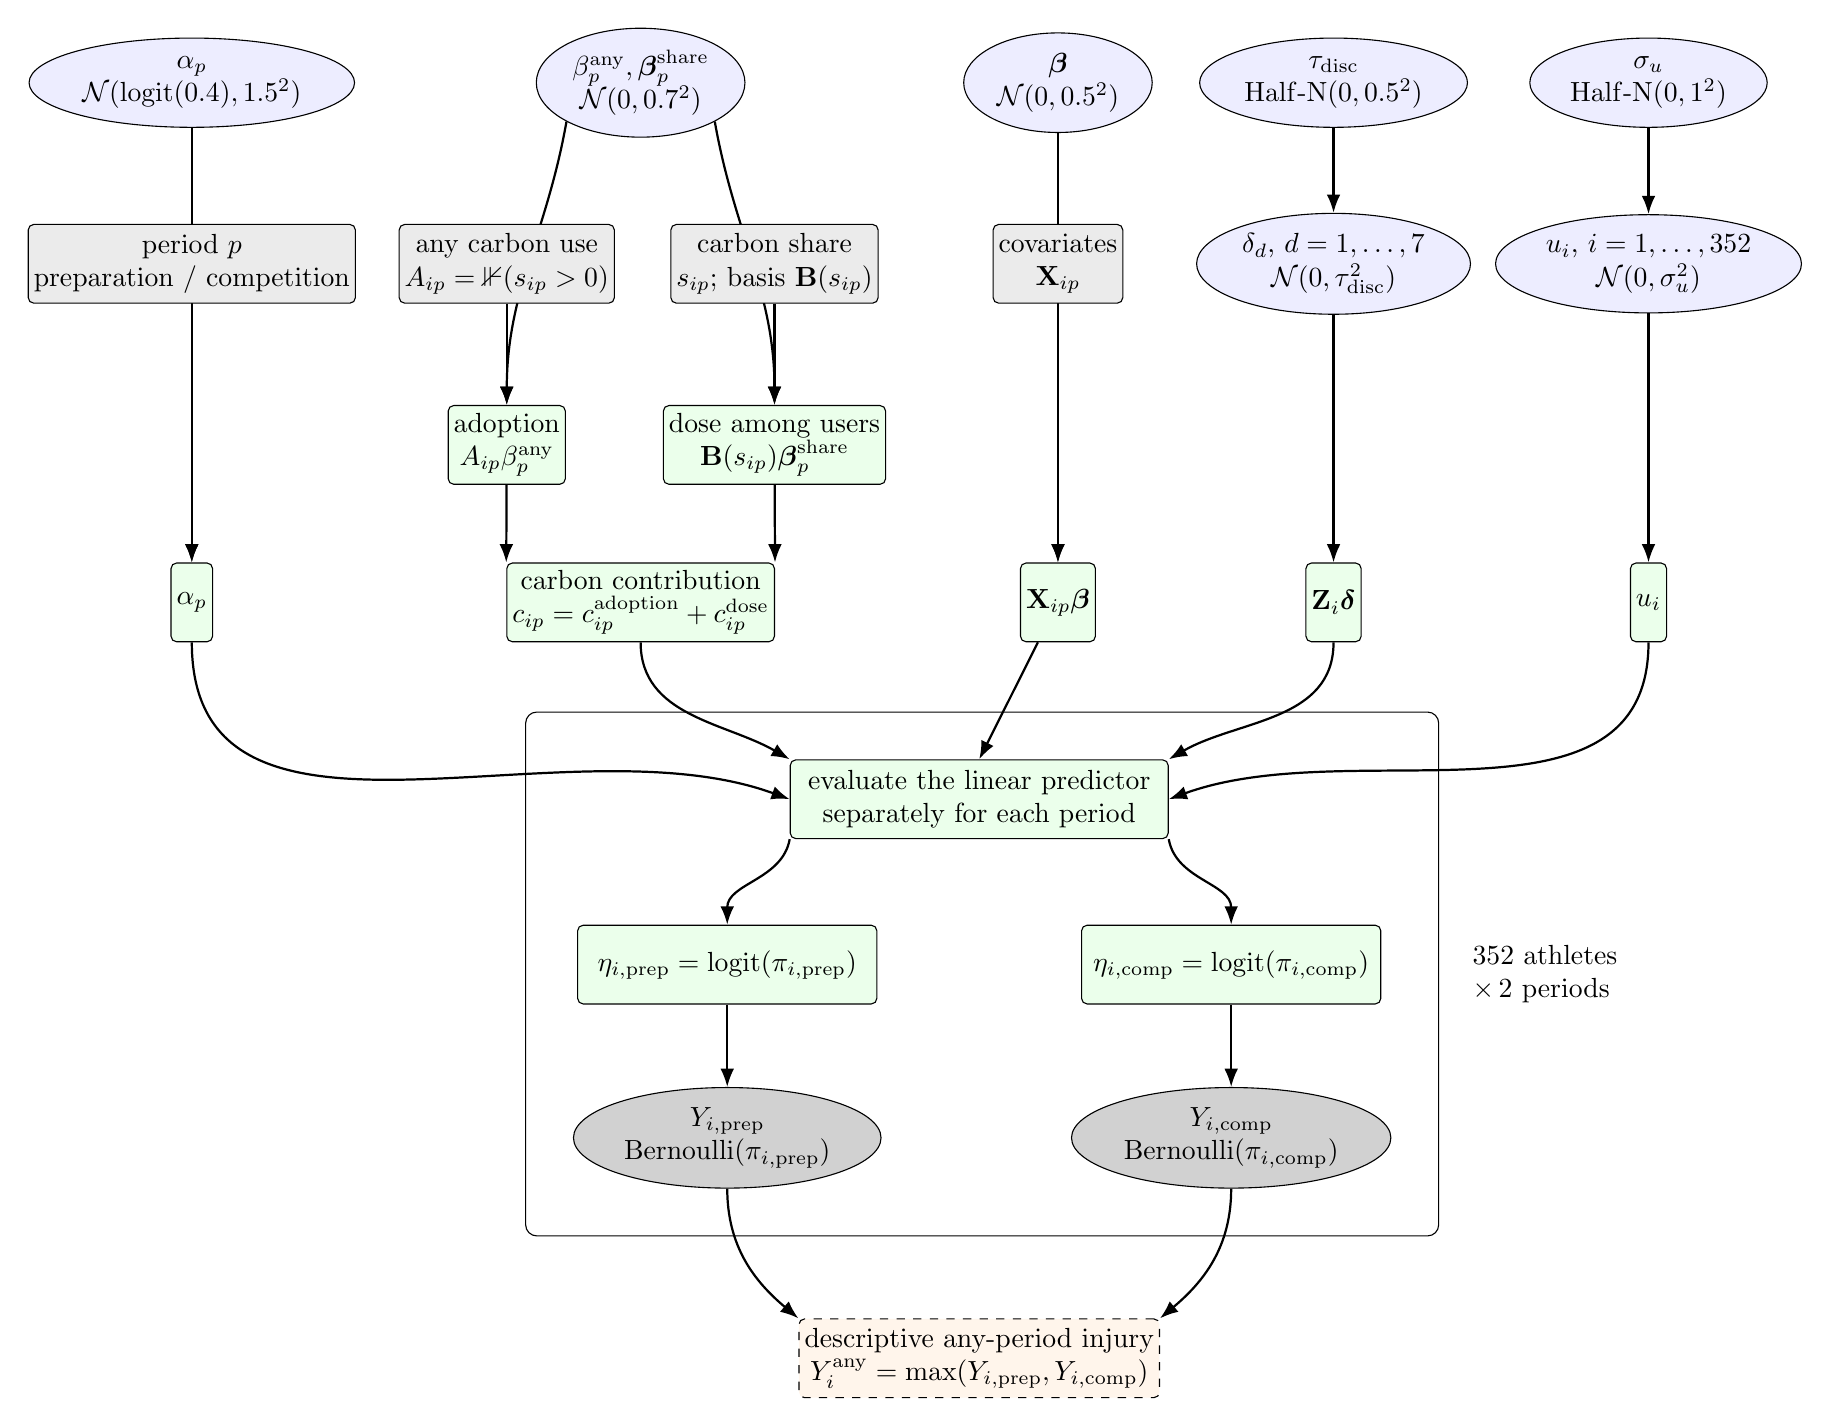
\begin{tikzpicture}[
  >=Latex,
  every node/.style={font=\normalsize},
  latent/.style={draw, ellipse, fill=blue!7, minimum height=10mm, align=center, inner sep=2pt},
  data/.style={draw, rounded corners=2pt, fill=black!8, minimum height=10mm, align=center, inner sep=2pt},
  term/.style={draw, rounded corners=2pt, fill=green!8, minimum height=10mm, align=center, inner sep=2pt},
  outcome/.style={draw, ellipse, fill=black!18, minimum height=12mm, align=center, inner sep=2pt},
  summary/.style={draw, dashed, rounded corners=2pt, fill=orange!8, minimum height=10mm, align=center, inner sep=2pt},
  plate/.style={draw, rounded corners=4pt, inner sep=6mm},
  arrow/.style={->, thick}
]


  \node[latent]                  (alpha)        at (-1.0, 0)     {$\alpha_p$\\$\mathcal N(\operatorname{logit}(0.4),1.5^2)$};
  \node[latent]                  (exposurecoef) at (4.7, 0)      {$\beta^{\mathrm{any}}_p,\boldsymbol\beta^{\mathrm{share}}_p$\\$\mathcal N(0,0.7^2)$};
  \node[latent]                  (commoncoef)   at (10.0, 0)     {$\boldsymbol\beta$\\$\mathcal N(0,0.5^2)$};
  \node[latent]                  (discscale)    at (13.5, 0)     {$\tau_{\mathrm{disc}}$\\$\operatorname{Half\text{-}N}(0,0.5^2)$};
  \node[latent]                  (athscale)     at (17.5, 0)     {$\sigma_u$\\$\operatorname{Half\text{-}N}(0,1^2)$};


  \node[data]                    (period)       at (-1.0, -2.3)  {period $p$\\preparation / competition};
  \node[data]                    (adoptioninput) at (3.0, -2.3)  {any carbon use\\$A_{ip}=\mathbb 1(s_{ip}>0)$};
  \node[data]                    (doseinput)     at (6.4, -2.3)  {carbon share\\$s_{ip}$; basis $\mathbf B(s_{ip})$};
  \node[data]                    (covariates)   at (10.0, -2.3)  {covariates\\$\mathbf X_{ip}$};
  \node[latent]                  (disccoef)     at (13.5, -2.3)  {$\delta_d$, $d=1,\ldots,7$\\$\mathcal N(0,\tau_{\mathrm{disc}}^2)$};
  \node[latent]                  (athleteeffect) at (17.5, -2.3) {$u_i$, $i=1,\ldots,352$\\$\mathcal N(0,\sigma_u^2)$};


  \node[term]                    (adoptionterm) at (3.0, -4.6)   {adoption\\$A_{ip}\beta^{\mathrm{any}}_p$};
  \node[term]                    (doseterm)     at (6.4, -4.6)   {dose among users\\$\mathbf B(s_{ip})\boldsymbol\beta^{\mathrm{share}}_p$};


  \node[term]                    (interceptterm)  at (-1.0, -6.6) {$\alpha_p$};
  \node[term]                    (exposureterm)   at (4.7, -6.6)  {carbon contribution\\$c_{ip}=c^{\mathrm{adoption}}_{ip}+c^{\mathrm{dose}}_{ip}$};
  \node[term]                    (covariateterm)  at (10.0, -6.6) {$\mathbf X_{ip}\boldsymbol\beta$};
  \node[term]                    (discterm)       at (13.5, -6.6) {$\mathbf Z_i\boldsymbol\delta$};
  \node[term]                    (athleteterm)    at (17.5, -6.6) {$u_i$};


  \node[term, minimum width=48mm] (periodassembly) at (9.0, -9.1)
    {evaluate the linear predictor\\separately for each period};

  \node[term, minimum width=38mm] (etaprep) at (5.8, -11.2)
    {$\eta_{i,\mathrm{prep}}=\operatorname{logit}(\pi_{i,\mathrm{prep}})$};
  \node[term, minimum width=38mm] (etacomp) at (12.2, -11.2)
    {$\eta_{i,\mathrm{comp}}=\operatorname{logit}(\pi_{i,\mathrm{comp}})$};


  \node[outcome] (prepoutcome) at (5.8, -13.4) {$Y_{i,\mathrm{prep}}$\\$\operatorname{Bernoulli}(\pi_{i,\mathrm{prep}})$};
  \node[outcome] (compoutcome) at (12.2, -13.4) {$Y_{i,\mathrm{comp}}$\\$\operatorname{Bernoulli}(\pi_{i,\mathrm{comp}})$};


  \node[summary] (anyoutcome) at (9.0, -16.2) {descriptive any-period injury\\$Y_i^{\mathrm{any}}=\max(Y_{i,\mathrm{prep}},Y_{i,\mathrm{comp}})$};

  \begin{pgfonlayer}{background}

    \draw[arrow] (alpha) -- (interceptterm);
    \draw[arrow] (period) -- (interceptterm);


    \draw[arrow] (exposurecoef.south west) to[out=-100,in=90] (adoptionterm.north);
    \draw[arrow] (exposurecoef.south east) to[out=-80,in=90] (doseterm.north);
    \draw[arrow] (adoptioninput) -- (adoptionterm);
    \draw[arrow] (doseinput) -- (doseterm);
    \draw[arrow] (adoptionterm) -- (exposureterm.north west);
    \draw[arrow] (doseterm) -- (exposureterm.north east);


    \draw[arrow] (commoncoef) -- (covariateterm);
    \draw[arrow] (covariates) -- (covariateterm);


    \draw[arrow] (discscale) -- (disccoef);
    \draw[arrow] (disccoef) -- (discterm);


    \draw[arrow] (athscale) -- (athleteeffect);
    \draw[arrow] (athleteeffect) -- (athleteterm);


    \draw[arrow] (interceptterm.south) to[out=-90,in=160] (periodassembly.west);
    \draw[arrow] (exposureterm.south) to[out=-90,in=150] (periodassembly.north west);
    \draw[arrow] (covariateterm) -- (periodassembly.north);
    \draw[arrow] (discterm.south) to[out=-90,in=30] (periodassembly.north east);
    \draw[arrow] (athleteterm.south) to[out=-90,in=20] (periodassembly.east);


    \draw[arrow] (periodassembly.south west) to[out=-100,in=90] (etaprep.north);
    \draw[arrow] (periodassembly.south east) to[out=-80,in=90] (etacomp.north);

    \draw[arrow] (etaprep) -- (prepoutcome);
    \draw[arrow] (etacomp) -- (compoutcome);


    \draw[arrow] (prepoutcome.south) to[out=-90,in=140] (anyoutcome.north west);
    \draw[arrow] (compoutcome.south) to[out=-90,in=40] (anyoutcome.north east);
  \end{pgfonlayer}

  \node[plate, fit=(periodassembly)(etaprep)(etacomp)(prepoutcome)(compoutcome)] (modelplate) {};
  \node[anchor=west, align=left] at ([xshift=3mm]modelplate.east) {$352$ athletes\\$\times\,2$ periods};
\end{tikzpicture}%
}
\caption{Graphical representation of the primary Bayesian multilevel model. Grey boxes are observed inputs, blue ellipses are estimated parameters, green boxes are deterministic contributions to the linear predictor, and shaded ellipses are the two observed period-specific injury outcomes, jointly enclosed in the solid plate (352 athletes $\times$ 2 periods). The carbon contribution $c_{ip}$ combines adoption ($A_{ip}$, any carbon use) and dose ($\mathbf B(s_{ip})$, the centered three-degree-of-freedom natural-spline basis for carbon share among users). $\mathbf Z_i$ denotes the seven discipline indicators underlying the partially pooled coefficients $\delta_d$, and $u_i$ the shared athlete random intercept. The common model structure is evaluated separately as $\eta_{i,\mathrm{prep}}$ and $\eta_{i,\mathrm{comp}}$; each predictor points only to its corresponding outcome. The dashed box is the derived any-period injury indicator reported descriptively, outside the probabilistic-model plate, and is not an additional likelihood term.}
\label{fig:primary-model-graph}
\end{figure}


\subsubsection{Estimands and marginal standardization}
\label{sec:estimands}
Posterior draws were used to compute marginal (population-standardized) adjusted prevalences by averaging model predictions over the observed empirical distribution of covariates and discipline indicators within each period, and by integrating the athlete random intercept using 15-point Gauss--Hermite quadrature rather than conditioning on a fixed value of $u_i$. For each period, adjusted prevalence was computed at four exposure scenarios: non-user, and user at the empirical 25th (P25), 50th (P50), and 75th (P75) percentile of the observed among-user share distribution for that period. These are ranks in the observed exposure distribution, not fixed share values: P25, P50, and P75 corresponded to 28.6\%, 42.1\%, and 57.1\% share in preparation and to 36.0\%, 50.0\%, and 71.4\% share in competition. Two primary contrasts were derived: the \emph{adoption} contrast (P50 user vs.\ non-user; prevalence difference and ratio) and the \emph{dose} contrast (P75 vs.\ P25 among users; prevalence difference and ratio).

To provide a directly interpretable absolute-risk presentation without fitting an additional model, the same posterior draws were also evaluated for one fixed reference profile. The profile was a male speed athlete aged 21 years, 176~cm tall, weighing 64~kg, with 10 years of athletics experience and an injury in either of the two preceding seasons. The period-matched training-frequency scores were fixed at their pooled cohort medians: long endurance 1, medium endurance 1, lactate 2, maximum velocity 2, technique 2, and gym 2; these are the survey's ordinal frequency scores, not exact counts of unique sessions. The athlete random intercept was fixed at zero (the median of its modeled distribution). Thus, ``median profile'' denotes medians for continuous and ordinal covariates combined with the modal observed sex and discipline profile, not a uniquely defined median athlete. Adoption was summarized as the risk difference between a non-user and a user at 50\% carbon share. Among users, the continuous HSGP risk curve was evaluated over the share range supported in both periods, with preparation and competition predictions calculated for this identical profile.

For display only, each continuous curve was read at three exact share values: 25\%, 50\%, and 75\%. These values are not P25, P50, and P75 of the sample, do not define exposure groups, and are not proposed clinical thresholds. They were selected after model fitting as round, evenly spaced interpretive anchors within the observed support of both periods; 50\% is also the pooled median user share and the centering point of the HSGP curve, while 25\% and 75\% are symmetric around it. A change from 25\% to 50\%, or from 50\% to 75\%, therefore means changing the carbon component from one-quarter to one-half, or from one-half to three-quarters, of the same fixed total reported training-frequency score for the same reference profile. Both changes are derived from one continuous fitted function, not from separate models or comparisons between athlete subgroups. These are conditional, profile-specific model predictions intended to aid interpretation of the fitted association, not validated individual prognostic estimates.

\subsubsection{Matched comparison of relative and absolute exposure}
\label{sec:exposure-scale-comparison}
To examine whether the observed association was specific to relative allocation or instead tracked absolute carbon use, two matched multilevel models represented two substantive exposure hypotheses. The \emph{relative-use hypothesis} used carbon share and asks whether injury prevalence changes as a greater proportion of a given training-frequency total is allocated to carbon-plated spikes. The \emph{absolute-use hypothesis} used the absolute carbon-frequency score and asks whether injury prevalence changes with more reported carbon use after adjustment for the same total training-frequency covariates. Both exposures were standardized among users across both periods (mean 0, standard deviation 1) and entered linearly with period-specific coefficients; each model also retained the period-specific adoption term, identical covariates, discipline effects, priors, and athlete random-intercept structure of the primary model. One standard deviation represented 0.241 in share (24.1 percentage points) or 3.36 units of the summed ordinal carbon-frequency score. The latter is a change in the questionnaire-derived score, not 3.36 unique training sessions, because frequency categories were top-coded and training domains could overlap within a session. The two exposures were fitted in separate models because absolute carbon frequency contributes directly to both the share numerator and the adjusted total-frequency scores; simultaneous inclusion would make the coefficients difficult to identify and interpret.

For a common conditional estimand, posterior injury risk was evaluated from 0.5 standard deviations below to 0.5 standard deviations above the pooled user mean. On the observed scales, this one-standard-deviation increase was from 37.3\% to 61.4\% carbon share or from 2.83 to 6.19 units of the summed ordinal carbon-frequency score. Continuous covariates were fixed at their cohort medians, discipline at the most prevalent observed indicator, and the athlete random intercept at zero. The comparison was designed to place the two scales on equal footing, not to treat absence of an association in one model as proof of no effect or to select a causal exposure mechanism. This matched exposure-scale comparison was added to clarify interpretation of the primary share analysis and was not part of the prospectively specified sensitivity set.

\subsubsection{Validation and sensitivity analyses}
\label{sec:validation}
Predictive comparison between the primary (exposure) and baseline (no-exposure) models used Pareto-smoothed importance-sampling leave-one-out cross-validation (PSIS-LOO) \citep{vehtari2017loo}, computed on the athlete-grouped joint log-likelihood (both period records per athlete evaluated jointly, with the athlete random intercept marginalized by Gauss--Hermite quadrature before leave-one-athlete-out prediction), reported as the expected log predictive density (ELPD) difference with its standard error. Posterior predictive checks compared observed and model-replicated counts of injured athletes per period. Two pre-specified sensitivity analyses tested structural assumptions of the primary specification: (1) a linear carbon-share term in place of the HSGP curve; (2) wider hyperpriors (HSGP marginal standard deviation $\alpha^{\text{gp}}_p \sim \text{Half-N}(0, 1.2^2)$, covariate coefficients $\mathcal{N}(0, 1.0^2)$, length-scale prior unchanged). Sensitivity models were compared with the primary model as robustness checks on the same estimands, not as competing substantive hypotheses.

\subsection{Population reweighting}
\label{sec:weighting}
Because the two-phase recruitment (Section~\ref{sec:participants}) could not guarantee equal selection probabilities across age-by-sex strata, a poststratification step \citep{gelman2007poststrat} reweighted the analysis sample to FIDAL national population estimates for six age-by-sex strata (Under 20, Under 23, Senior $\times$ Men, Women; Appendix Table~\ref{tab:weight-diagnostics}). Stratum model weights were the ratio of the population share to the observed sample share, further regularized to avoid extreme weights. The Kish effective sample size after weighting was 340.5 of 352 (97\%), indicating a modest efficiency loss from reweighting. Weighted estimands were computed by combining the athlete-level posterior predictions of Section~\ref{sec:estimands} with model weights before marginalization, and are reported alongside the unweighted (sample-representative) estimands as a sensitivity check on generalizability to the national competitive population.

\subsection{Subgroup analyses}
\label{sec:subgroups}
As a pre-specified descriptive and exploratory extension, the primary adjusted estimands were recomputed conditional on sex (men, women) and on age group (Under 20, Under 23, Senior), holding the same model structure and covariate adjustment, to assess whether the direction and approximate magnitude of the competition-period dose association were consistent across these strata. These subgroup estimates are not powered as confirmatory tests of effect-modification and are reported as descriptive, hypothesis-generating comparisons.

\subsection{Sources of bias}
\label{sec:bias}
The survey instrument underwent content-validity and face-validity review by athletics-medicine content experts and prospective respondents before deployment, but no formal test-retest reliability or criterion-validity assessment against objectively measured training data (for example, coach-logged sessions or shoe-embedded wear sensors) was conducted; this is treated as a limitation rather than a validated measurement property (Section~\ref{sec:discussion-limitations}). Both exposure and outcome were self-reported for the same recall period by the same respondent, which admits recall bias and the possibility that athletes' beliefs about carbon-plate risk influenced how they reported either quantity. The survey was administered near the end of the competitive season, so the competition-period recall window was recent while the preparation-period window reached further back into the season; this asymmetry is a plausible source of differential, period-specific recall error, and any resulting attenuation in preparation-period exposure and outcome reporting would bias that period's association toward the null independently of the underlying biomechanics. This offers one plausible explanation, among others, for why the preparation-period association was weaker and less certain than the competition-period one, and is a reason to treat the period contrast itself, not only the individual period estimates, with some caution. Reporting was not restricted to medically trained staff; athletes reported their own injuries and training without independent clinical verification, following the broad, non-medical-attention-dependent injury definition of Section~\ref{sec:outcome}, which was chosen specifically to reduce under-ascertainment of injuries that did not prompt a clinical visit at the cost of relying on athlete-reported symptom recognition rather than diagnosis.

\subsection{Missing data and other analyses}
\label{sec:missing}
The analysis used a complete-case cohort by design: eligibility required a fully completed survey, and the three further exclusions in Section~\ref{sec:participants} addressed incomplete injury timing or a structurally undefined carbon-share denominator. No further imputation was performed.

\subsection{Software}
\label{sec:software}
The fitted models used a Bernoulli likelihood with a logit link. Posterior sampling used Stan's No-U-Turn Sampler (NUTS), a Hamiltonian Monte Carlo algorithm, through the \texttt{rstan} interface. For each model, four independent chains each ran for 2000 iterations; the first 1000 were used for warm-up and adaptation and discarded, leaving 1000 retained draws per chain and 4000 retained draws in total to approximate the posterior distribution. The target acceptance probability was set to \texttt{adapt\_delta}=0.98 and the maximum tree depth to 12. Runs used base seed 20260719 with deterministic model-specific offsets. Analyses used the \texttt{loo} package for PSIS-LOO cross-validation; the HSGP basis, spectral density, and length-scale prior calibration were implemented directly in Stan and base R, with no additional package dependency. Full software versions are reported in Appendix~\ref{sec:session-info}.


\section{Results}
\label{sec:results}
\subsection{Sample flow and recruitment}
\label{sec:results-flow}
Table~\ref{tab:sample-flow} summarizes the flow from survey completion to the balanced analysis cohort of 352 athletes and 704 athlete-period records. Phase 2 targeted recall concentrated additional enrollment in Under 20 and Under 23 strata, particularly hurdles, horizontal jumps, and combined events, which the voluntary Phase 1 sample under-represented relative to the FIDAL population estimate. After poststratification (Section~\ref{sec:weighting}; Appendix Table~\ref{tab:weight-diagnostics}), the Kish effective sample size was 340.5 of 352 analyzed athletes (97\%), indicating that reweighting did not substantially inflate posterior uncertainty.

\subsection{Baseline characteristics}
\label{sec:results-table1}
Table~\ref{tab:table1} compares baseline characteristics by competition sex, the principal descriptive contrast for this cohort, alongside the corresponding population-weighted standardized mean differences (SMD). As expected for a sex comparison, height and weight showed large SMDs ($-1.81$ and $-1.83$); demographic, injury-history, carbon-exposure, and discipline-distribution SMDs were mostly below the conventional 0.20 threshold for a small imbalance \citep{table1guidelines}, with horizontal jumps and combined events showing modest over-representation of women (SMD 0.22--0.23). Reweighting to national population strata (weighted SMD column) did not materially change this pattern, supporting the sample as broadly representative of the target competitive population once poststratified.

\subsection{Descriptive carbon-plate insole use}
\label{sec:results-descriptive}
Across the balanced cohort, carbon-plated spikes accounted for a mean 35.7\% of reported preparation-period training-type frequency and 47.7\% of reported competition-period training-type frequency (Table~\ref{tab:descriptive-carbon}). This pattern--roughly two-fifths of preparation training and roughly half of competition training reported in carbon-plated spikes--was stable across sex and age-group strata (Table~\ref{tab:descriptive-carbon}, Figure~\ref{fig:descriptive-carbon-share-by-stratum}), with mean shares differing by at most 4 percentage points between men and women or across the three age groups in either period, and with the full distributions--not only their means--overlapping closely between strata. Adoption (any carbon use) was high in both periods: 81.5\% of athletes reported any preparation carbon use and 87.5\% reported any competition carbon use (Table~\ref{tab:table1}), consistent with carbon-plated spikes functioning as the prevailing rather than niche equipment choice in this population.

\subsection{Specialty-group-stratified characteristics}
\label{sec:results-discipline}
To summarize the seven disciplines with limited individual cell sizes (19--107 athletes; Appendix Table~\ref{tab:discipline-support}), they were collapsed into four broader, physiologically motivated specialty groups--sprint/hurdles, endurance (middle and long distance), jumps (horizontal jumps or pole vault), and combined events. Tables~\ref{tab:specialty-group} and~\ref{tab:specialty-group-carbon} report baseline characteristics, injury prevalence, and carbon-plate use by group. Because disciplines and, consequently, groups are multi-select, 26 of 352 athletes belong to more than one group. Two patterns stand out as original descriptive findings of this cohort.

First, competition-period carbon share tracked the explosive-versus-endurance character of the group rather than being uniform across athletics. The sprint/hurdles group (the largest, $n=169$) had the highest competition carbon share (0.56) and the largest preparation-to-competition rise (+0.17), while the endurance group ($n=109$) had the lowest carbon share in both periods (0.31 and 0.34). This is consistent with the biomechanical rationale in Section~\ref{sec:introduction}: carbon-plate stiffness benefits are most established for short-duration, high-power efforts, and this cohort's self-reported equipment allocation mirrors that distinction even though the survey did not ask athletes about performance rationale directly.

Second, injury prevalence did not track carbon share in the same way. The jumps group ($n=62$) stood out with the highest prior-injury history (83.9\%) and the highest competition-period injury prevalence (51.6\%) of the four groups, despite an intermediate carbon share (0.47)--higher than endurance but lower than sprint/hurdles--indicating that the elevated injury burden in jumping disciplines is unlikely to be explained by carbon-plate dose alone and more plausibly reflects the landing and eccentric loading demands specific to jumping events; the primary Bayesian model (Section~\ref{sec:results-primary}) already adjusts for discipline using partially pooled indicators specifically to avoid attributing this discipline-driven variation to carbon exposure. The combined-events group ($n=41$) showed a distinct hybrid profile: a carbon share close to sprint/hurdles (0.52) paired with an endurance-like training volume (preparation and competition medians of 9) and an elevated any-injury prevalence (70.7\%), consistent with the mixed physiological demands of multi-event competition and with the higher, more heterogeneous musculoskeletal load noted for plyometric and multi-skill disciplines in prior athletics injury literature \citep{edouard2020injury}.

\subsection{Injury location and type}
\label{sec:results-pattern}
The 204 injured athletes reported 259 injuries in total (149 athletes with one injury, 55 with two), a median of 1 injury per affected athlete. Table~\ref{tab:injury-location} reports the anatomical location of these injuries and Figure~\ref{fig:injury-location-type} displays both the location and type distributions together. The thigh was, by a substantial margin, the single most commonly reported location (97 of 259 injuries, 37.5\%; affecting 80 of 204 injured athletes, 39.2\%), followed by the lower leg (25.1\% of injuries) and the foot (19.3\%); together, the hip, groin, thigh, lower leg, ankle, and foot accounted for 95.8\% of all reported injuries, with only 4.2\% localized to the head, upper limb, or trunk.

For the 248 lower-limb injuries for which an injury type was recorded (Table~\ref{tab:injury-type}, Figure~\ref{fig:injury-location-type}), tendinopathy (28.6\%) and bone stress injury or stress fracture (26.2\%) were the two most frequently reported types, together accounting for more than half of classified lower-limb injuries and each individually more common than muscle strain (22.2\%). This is a distinctive feature of this cohort relative to general athletics injury surveillance, where muscle injury is typically the most frequently reported tissue type by a wide margin and tendon and bone injuries are reported considerably less often \citep{edouard2020injury}.

Cross-tabulating type against location (Table~\ref{tab:injury-type-by-location}) shows that these two leading types were not distributed the same way anatomically. Tendinopathy was disproportionately distal relative to the overall injury-location pattern: foot (35.2\% of the 71 tendinopathy injuries) and lower leg (33.8\%) were more prominent locations for tendinopathy than for the injury sample as a whole (19.3\% and 25.1\% respectively; Table~\ref{tab:injury-location}), and ankle involvement (22.5\%) was likewise higher than the sample-wide 13.9\%--a pattern compatible with Achilles- and plantar-tendon structures at the distal lower limb, consistent with the biomechanical literature on carbon-plate loading of the ankle and forefoot \citep{gerlach2025aft}. Bone stress injury or stress fracture, in contrast, was thigh-dominant (58.5\% of the 65 bone stress injuries), a pattern closely tracking the overall injury-location distribution and similar to muscle strain (74.5\% thigh) rather than being disproportionately distal; foot involvement among bone stress injuries (15.4\%) was, if anything, lower than the sample-wide rate. The elevated overall frequency of bone stress injury in this cohort is therefore a genuine descriptive finding, but this cohort's data do not show the foot/navicular-specific concentration that would most directly support the mechanistic link to carbon-plate loading proposed for that injury type \citep{tenforde2023bonestress}; the survey's type item does not further subclassify bone site (for example, navicular versus tibial versus metatarsal), so this distinction cannot be resolved further with the present data. Taken together, the location-by-type pattern strengthens the tendinopathy--carbon-plate hypothesis specifically, while leaving the bone-stress-injury hypothesis only partially supported. This is reported as a hypothesis-generating observation: the present cross-sectional design and sample size do not support a formal type-stratified test of the carbon-share association, and confirming a tendinopathy-specific association with carbon-plate dose, or resolving the anatomical site of the bone stress injuries observed here, would require a dedicated, adequately powered follow-up.

\subsection{Athlete-reported injury burden}
\label{sec:results-ostrc}
Of the 204 injured athletes, 193 (94.6\%) completed all four adapted OSTRC-H2 impact items. The median total severity score was 75 (IQR 58--92) overall (Table~\ref{tab:ostrc-period}). Scores were similar for athletes injured only during preparation (median 71.5, IQR 50--90) and only during competition (67, IQR 58--84; SMD $-0.07$), while athletes reporting injury in both periods had a higher median score of 84 (IQR 67--92; SMD 0.41 versus competition only). The largest component difference was for symptoms in the both-period group (SMD 0.51). These results describe impact among athletes already classified as injured; they are not a second injury-prevalence analysis.

\begin{table}[htbp]
\centering
\small
\caption{Adapted OSTRC-H2 impact scores among 193 injured athletes with complete responses, stratified by mutually exclusive injury period. Values are median [Q1, Q3]. Each component ranges from 0 to 25 and total severity from 0 to 100; higher scores indicate greater impact. SMDs compare group means with the competition-only group and are descriptive.}
\label{tab:ostrc-period}
\begin{tabular}{L{2.8cm}rrrrrr}
\toprule
& Overall & Preparation & Competition & Both & \multicolumn{2}{c}{SMD vs competition} \\
\cmidrule(lr){6-7}
Domain & ($n=193$) & only ($n=50$) & only ($n=84$) & periods ($n=59$) & Preparation & Both \\
\midrule
Participation & 17 [17, 25] & 17 [17, 25] & 17 [8, 25] & 17 [17, 25] & 0.14 & 0.19 \\
Training volume & 17 [17, 25] & 17 [8, 25] & 17 [8, 25] & 25 [17, 25] & 0.01 & 0.29 \\
Performance & 17 [17, 25] & 17 [8, 25] & 17 [17, 25] & 25 [17, 25] & $-0.35$ & 0.22 \\
Symptoms & 17 [8, 25] & 17 [8, 17] & 17 [8, 17] & 17 [17, 25] & $-0.01$ & 0.51 \\
Total severity & 75 [58, 92] & 71.5 [50, 90] & 67 [58, 84] & 84 [67, 92] & $-0.07$ & 0.41 \\
\bottomrule
\end{tabular}
\end{table}


\begin{figure}[htbp]
\centering
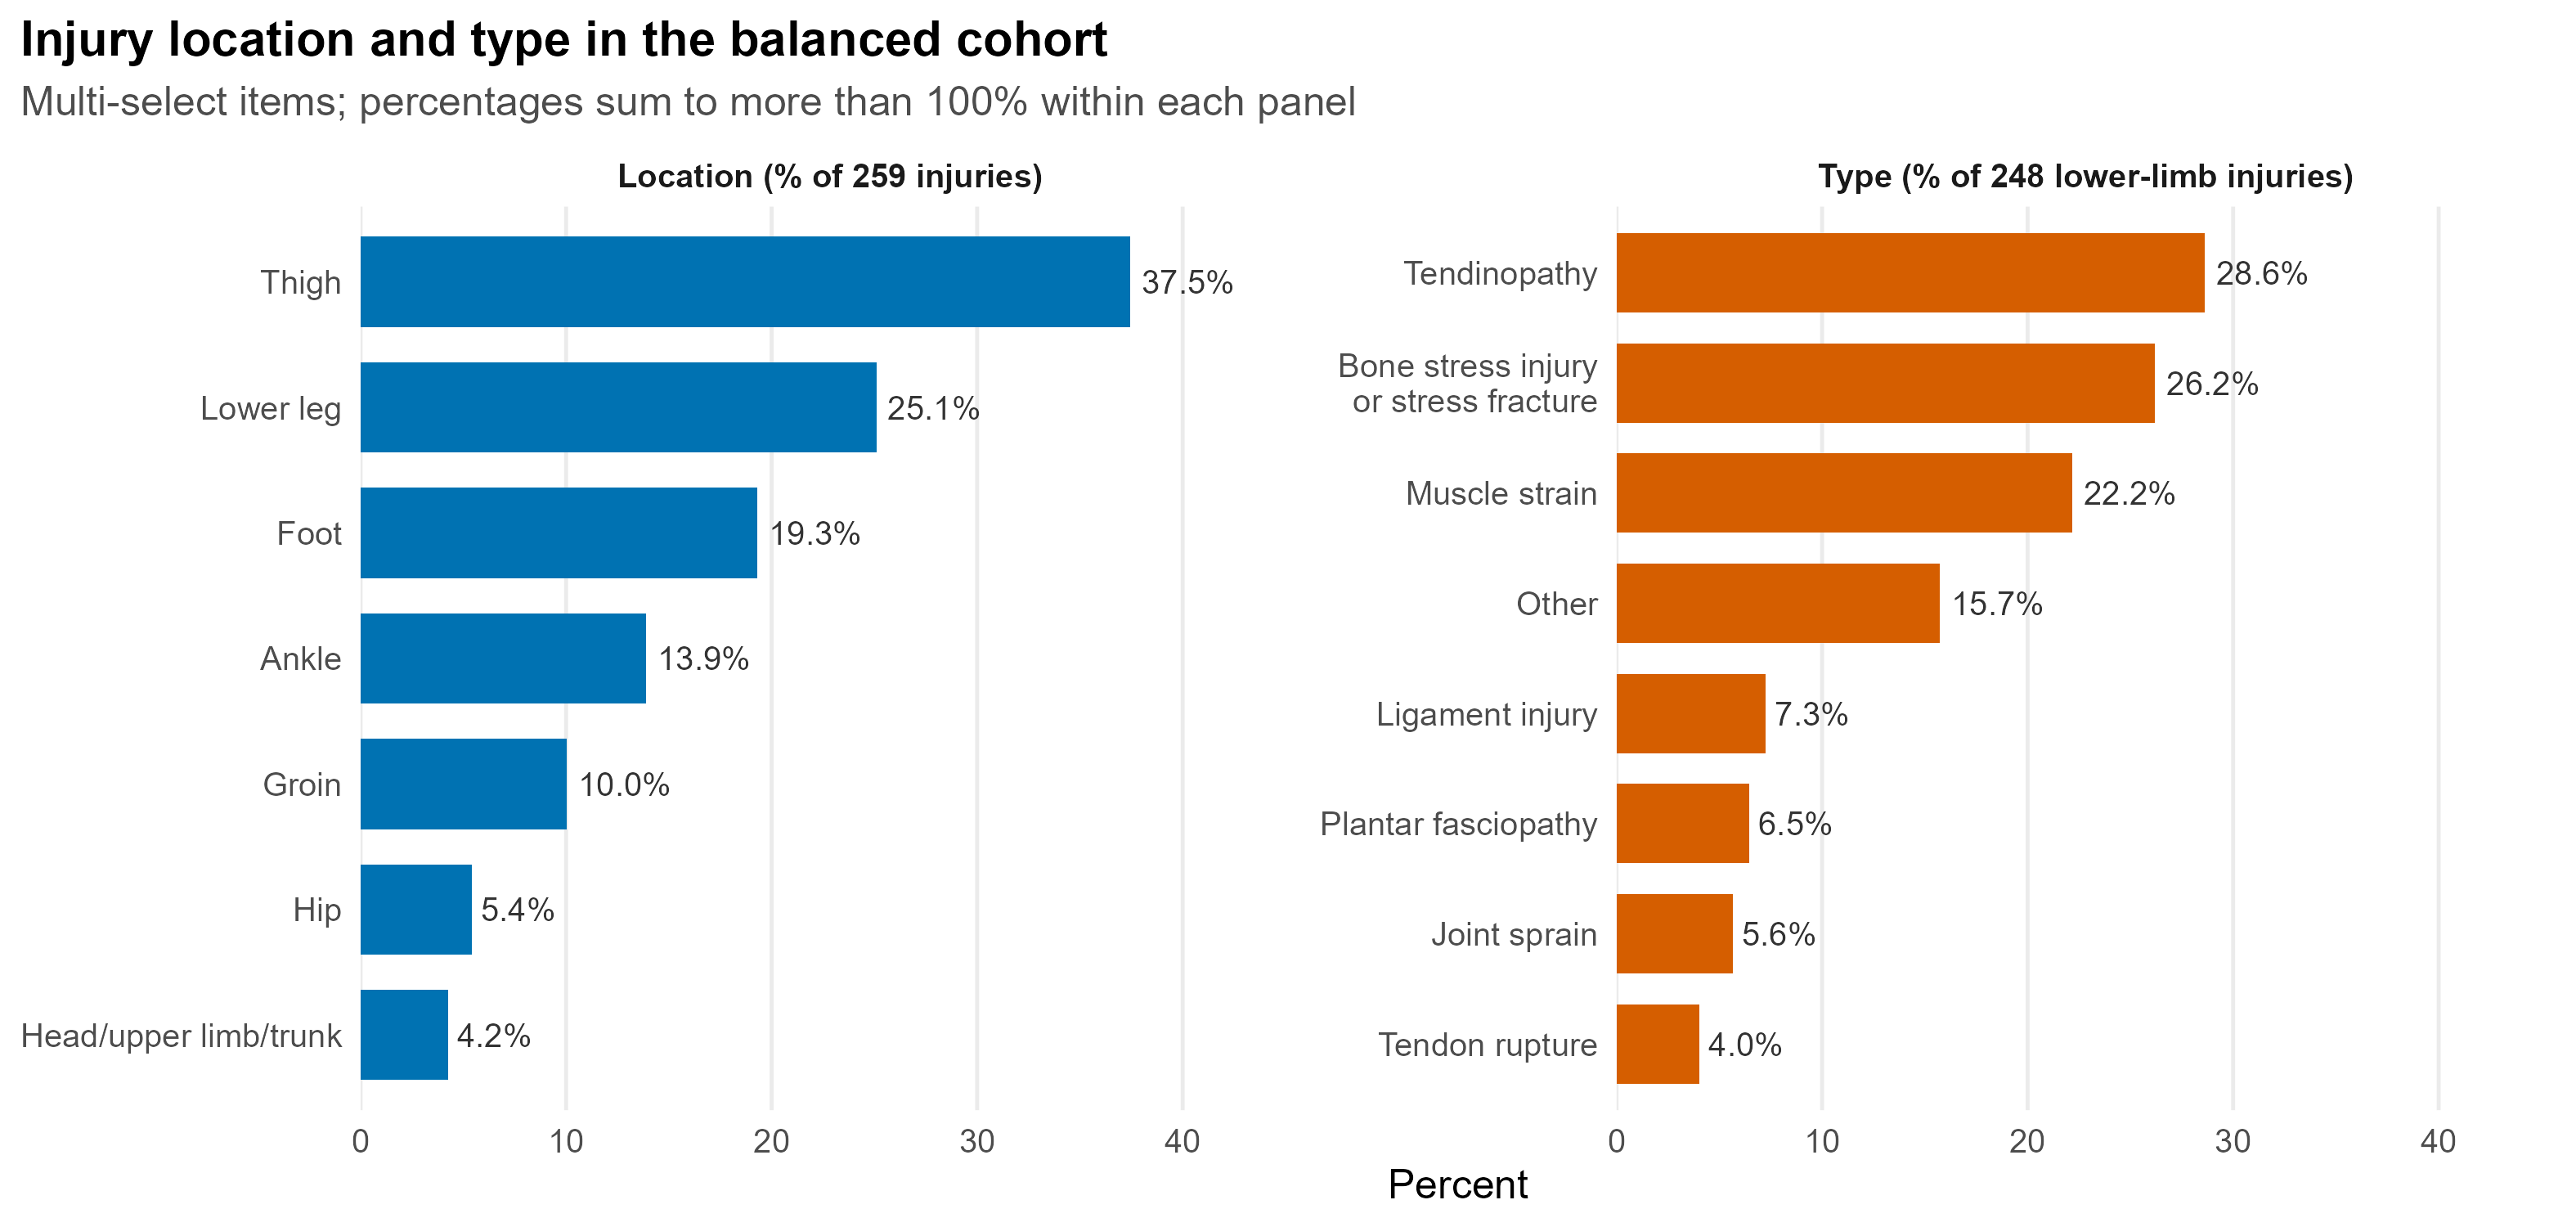
\includegraphics[width=0.95\textwidth]{fig_injury_location_type.png}
\caption{Anatomical location (\% of 259 injuries) and type (\% of 248 lower-limb injuries with a recorded type) of injuries reported by the balanced analysis cohort. Both items are multi-select, so percentages within each panel sum to more than 100\%.}
\label{fig:injury-location-type}
\end{figure}

\subsection{Primary adjusted associations}
\label{sec:results-primary}
Figure~\ref{fig:carbon-share-distribution} shows the observed distribution of carbon share by period; Figure~\ref{fig:spline-dose-response} displays the fitted among-user spline, and Figure~\ref{fig:posterior-associations} and Table~\ref{tab:primary-associations} summarize the primary adjusted estimands. Adjusted preparation-period injury prevalence was 30.1\% (95\% CrI 21.0--40.2\%) for non-users and 35.5\% (95\% CrI 29.6--41.7\%) for median-share users; the adoption difference of 5.4 percentage points (pp) (95\% CrI $-6.3$ to $16.2$) had a posterior probability of 82.0\% of being positive, well short of the threshold used here to describe an association as clear. The preparation-period dose contrast (75th vs.\ 25th percentile share among users) was $-0.8$ pp (95\% CrI $-10.6$ to $9.1$; posterior probability of a positive association 43.8\%), that is, centered near no association.

Adjusted competition-period injury prevalence was 38.1\% (95\% CrI 26.6--50.4\%) for non-users and 43.0\% (95\% CrI 36.5--49.4\%) for median-share users, an adoption difference of 4.8 pp (95\% CrI $-8.7$ to $17.7$; posterior probability 77.1\%). In contrast, among competition-period users, moving from the 25th percentile (36.0\% share) to the 75th percentile (71.4\% share) of carbon share was associated with adjusted prevalence rising from 36.0\% (95\% CrI 28.5--44.0\%) to 50.3\% (95\% CrI 42.4--58.2\%): a difference of 14.3 pp (95\% CrI 2.7 to 25.8) and a ratio of 1.41 (95\% CrI 1.06 to 1.86), with a posterior probability of 99.0\% that the association was positive and 94.0\% that it exceeded the pre-specified 5-pp threshold for a practically relevant association (Table~\ref{tab:primary-associations}). This competition-period dose association was the only one of the four primary contrasts for which the credible interval excluded zero.

\subsection{Model validation}
\label{sec:results-validation}
Both the primary (exposure) and matched baseline (no-exposure) models showed acceptable sampling behavior: maximum $\hat{R} \leq 1.003$, zero divergent transitions, zero maximum-tree-depth hits, and minimum E-BFMI above 0.66 in both models (Appendix Table~\ref{tab:model-comparison}). Posterior predictive checks reproduced the observed injury counts closely: the full posterior predictive distribution of replicated injured-athlete counts was centered on 115.5 (observed 115) for preparation and 149.5 (observed 149) for competition, with the observed count falling centrally within each replicated distribution (Figure~\ref{fig:posterior-predictive}). Every athlete-level PSIS-LOO Pareto-$k$ value was at most 0.5 in both models, supporting the reliability of the leave-one-out estimates. The exposure model's athlete-grouped ELPD exceeded the baseline model's by 2.22 (SE 2.30) (Appendix Table~\ref{tab:model-comparison}): the exposure terms did not clearly improve held-out predictive performance, even though the competition-period dose contrast itself had a high posterior probability of being positive. These two findings are compatible: a single, spline-parameterized, period-specific exposure effect concentrated in a subset of the competition-period users can produce a credible marginal association without moving whole-model out-of-sample predictive accuracy by a detectable amount in a cohort of this size.

\subsection{Sensitivity analyses}
\label{sec:results-sensitivity}
The direction of the competition-period dose association was stable across both pre-specified sensitivity analyses, but its magnitude was not (Table~\ref{tab:sensitivity}, Figure~\ref{fig:competition-dose-sensitivity}). Under a linear carbon-share parameterization, the association reduced to 6.0 pp (95\% CrI $-0.3$ to $12.6$; posterior probability 96.9\%), with the credible interval marginally including zero. Under wider priors, the association increased to 18.7 pp (95\% CrI 5.2 to 31.9; posterior probability 99.5\%). Taken together, the consistent positive direction across three structurally different specifications supports treating the competition-period dose association as a genuine feature of these data, while the sensitivity of its magnitude to the assumed dose--response shape argues against reporting 14.3 pp as a stable, precise effect size.

\subsection{Population-weighted and subgroup estimates}
\label{sec:results-weighted-subgroups}
After poststratification to national age--sex population strata, the competition-period dose association changed little: 14.9 pp (95\% CrI 3.3 to 26.4) weighted versus 14.3 pp (95\% CrI 2.7 to 25.8) unweighted (Appendix Table~\ref{tab:weighted-vs-unweighted}, Figure~\ref{fig:weighted-dose-by-sex}, Figure~\ref{fig:weighted-dose-by-age}). The two adoption contrasts and the preparation-period dose contrast likewise remained centered near no association after weighting. Conditional on sex or age group, the competition-period dose association retained a consistent point estimate (14.3--15.5 pp) and an essentially unchanged posterior probability of a positive association (99.4\% in every stratum examined; Appendix Table~\ref{tab:subgroups}), providing no descriptive evidence that the association was concentrated in, or specific to, a single sex or age-group stratum.

\begin{figure}[htbp]
\centering
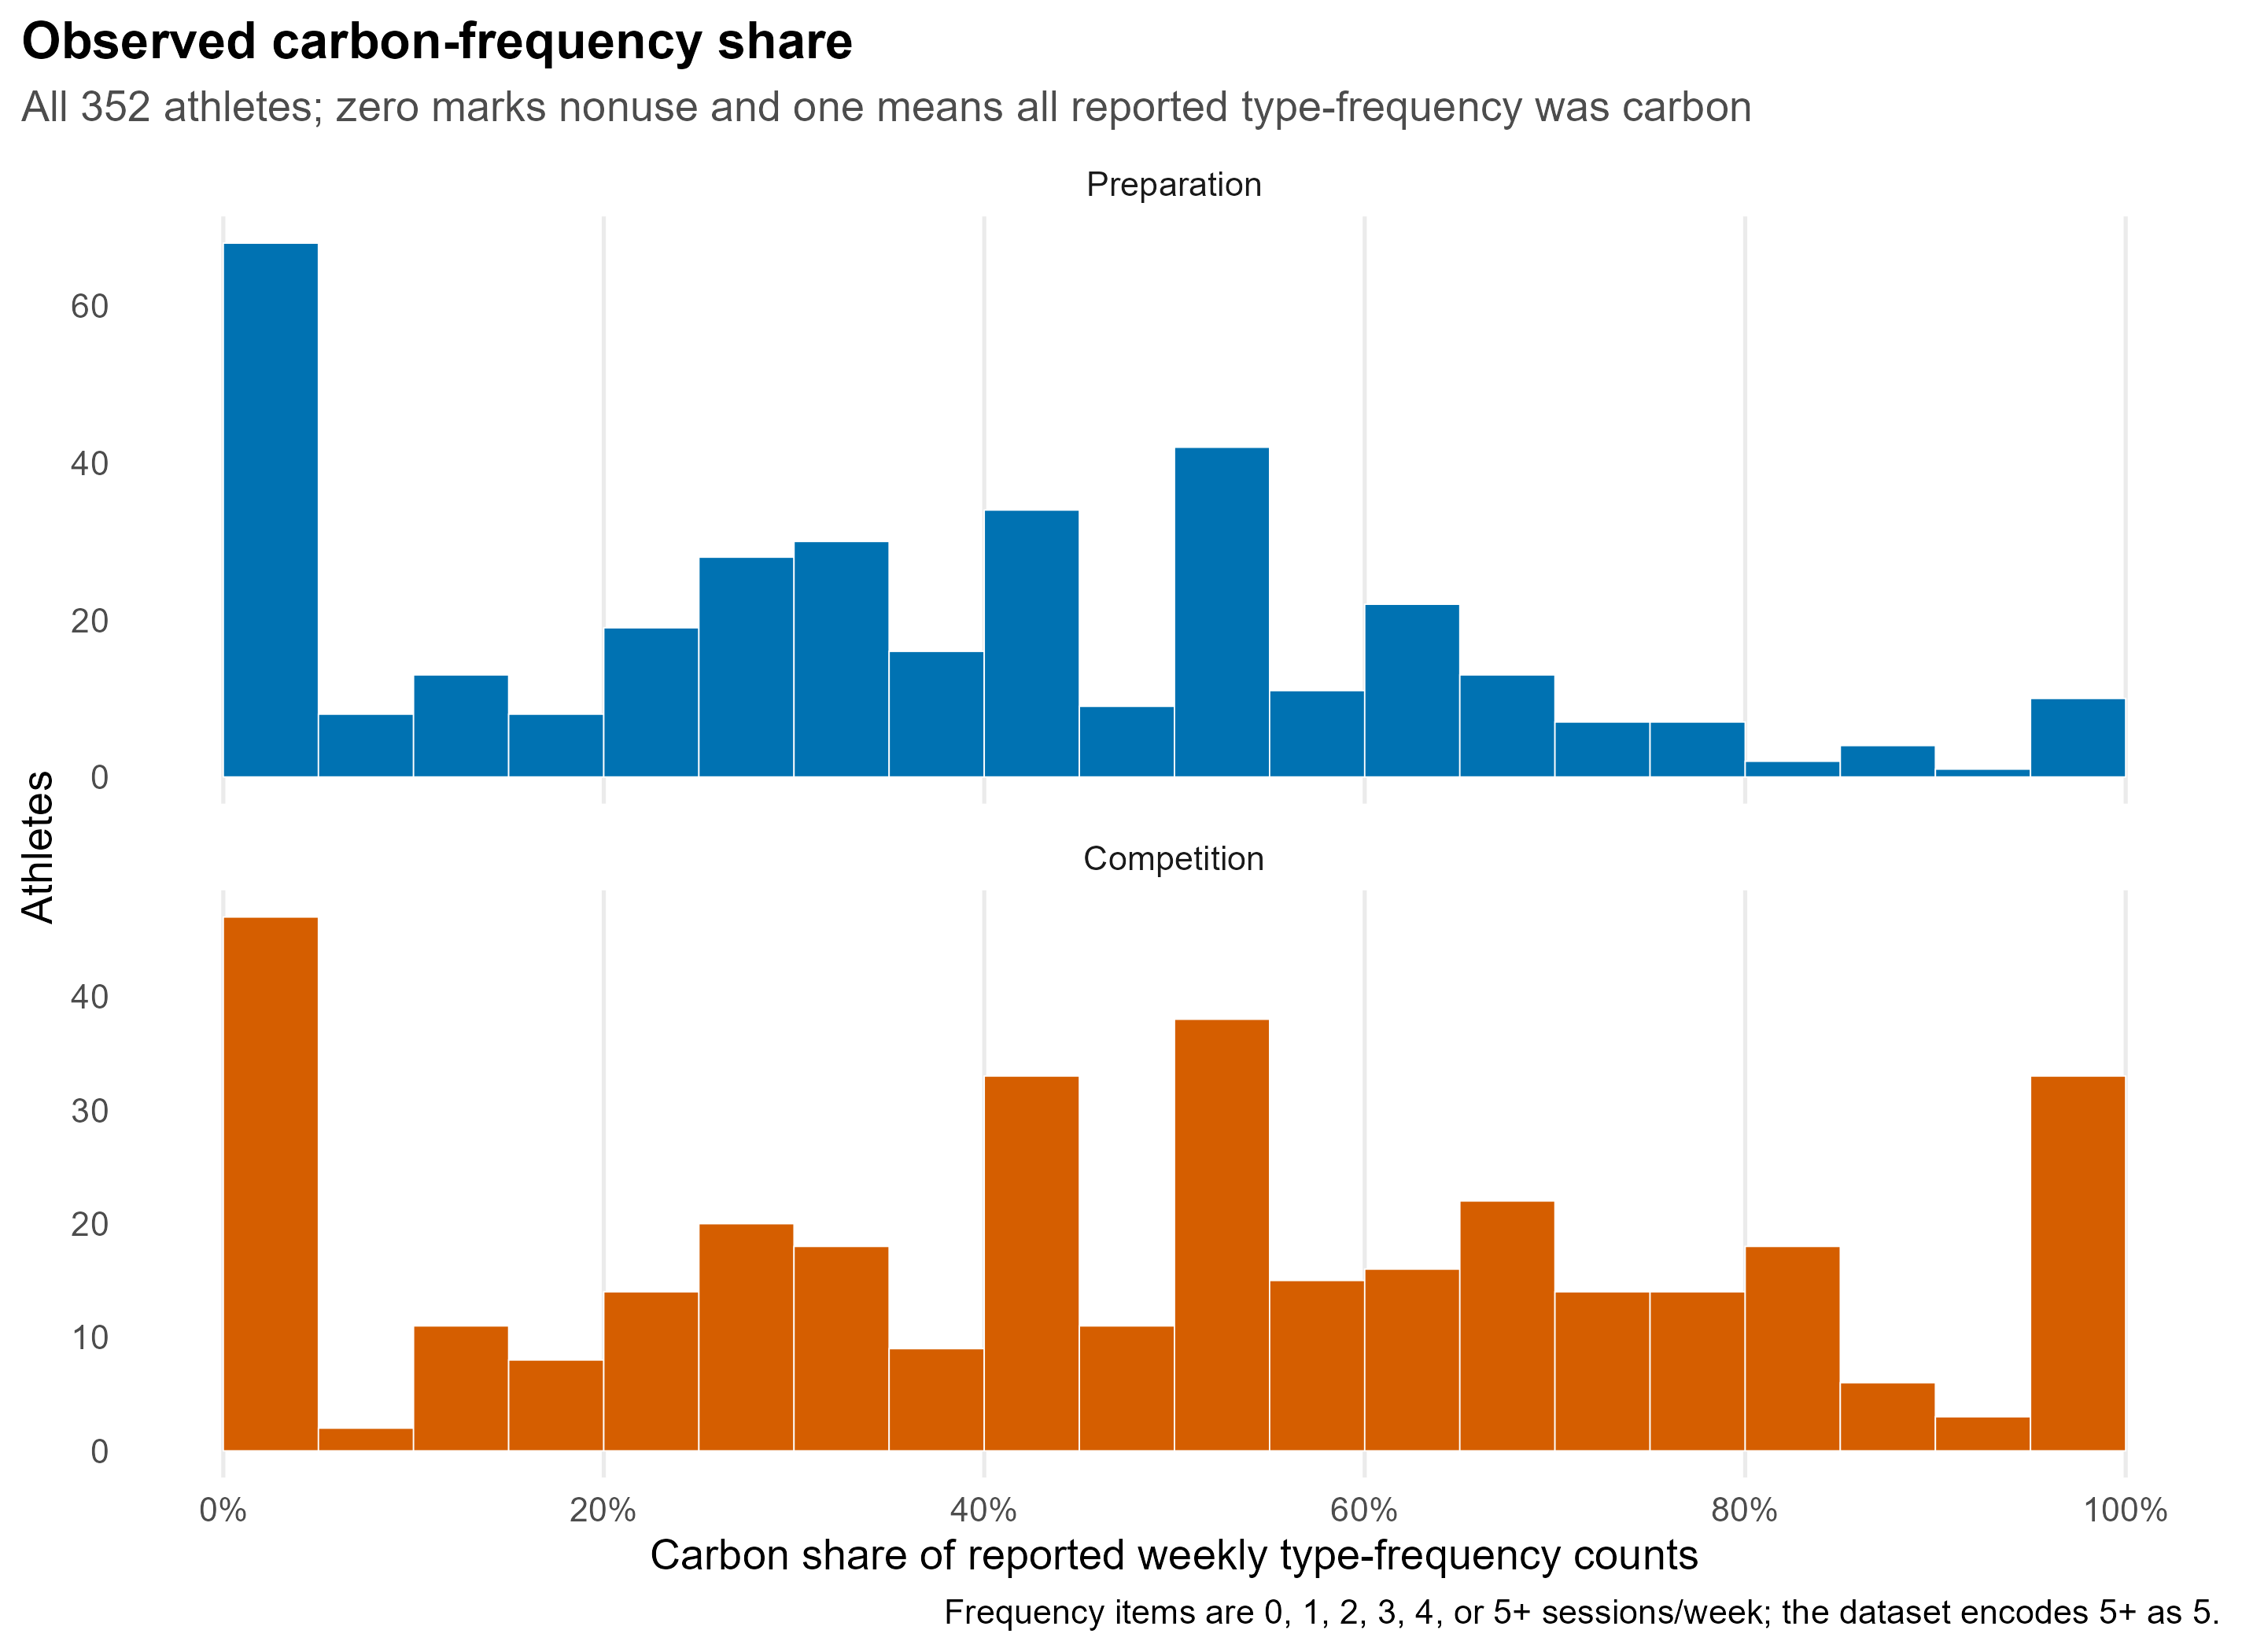
\includegraphics[width=0.85\textwidth]{fig_carbon_share_distribution.png}
\caption{Observed distribution of carbon-plate insole share of reported training-type frequency, among all 352 athletes, by period.}
\label{fig:carbon-share-distribution}
\end{figure}

\begin{figure}[htbp]
\centering
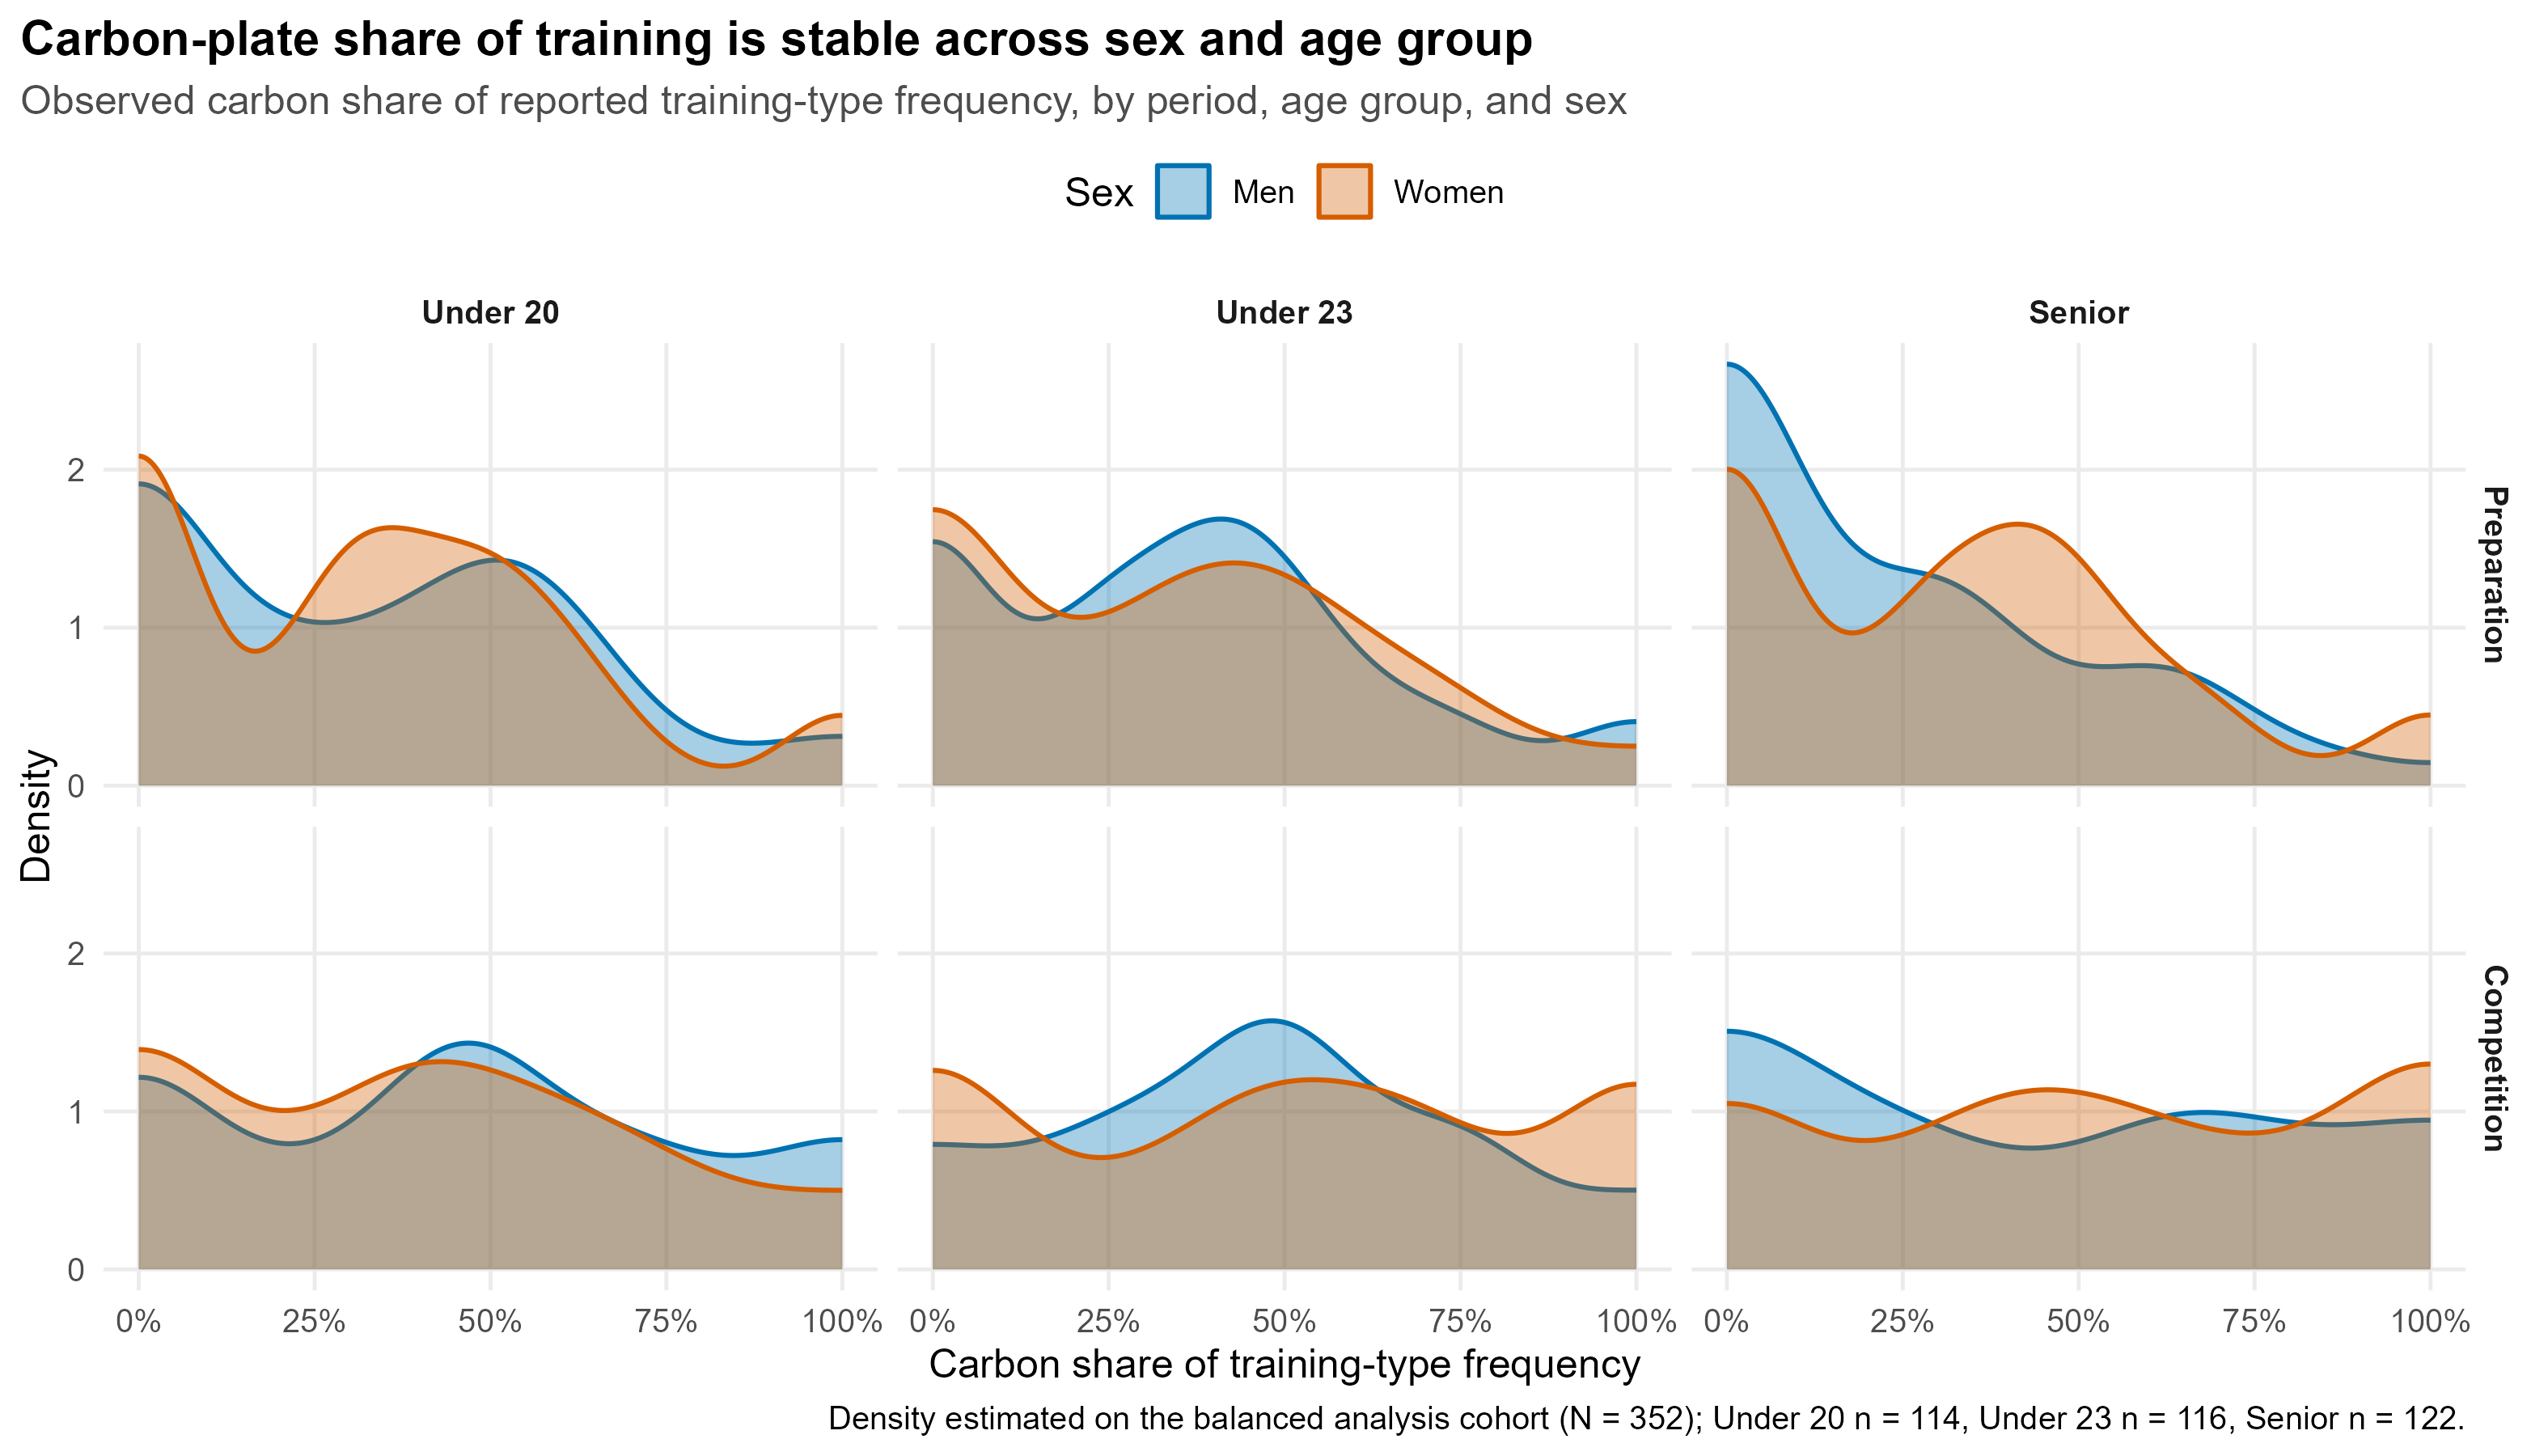
\includegraphics[width=0.95\textwidth]{fig_descriptive_carbon_share_by_stratum.png}
\caption{Observed distribution of carbon-plate insole share of reported training-type frequency, by period, age group, and sex. Curves are boundary-corrected kernel density estimates over the observed discrete-ratio share values (Section~\ref{sec:exposure}), shown to compare distributional overlap across strata; they are a smoothing device for visualization.}
\label{fig:descriptive-carbon-share-by-stratum}
\end{figure}

\begin{figure}[htbp]
\centering
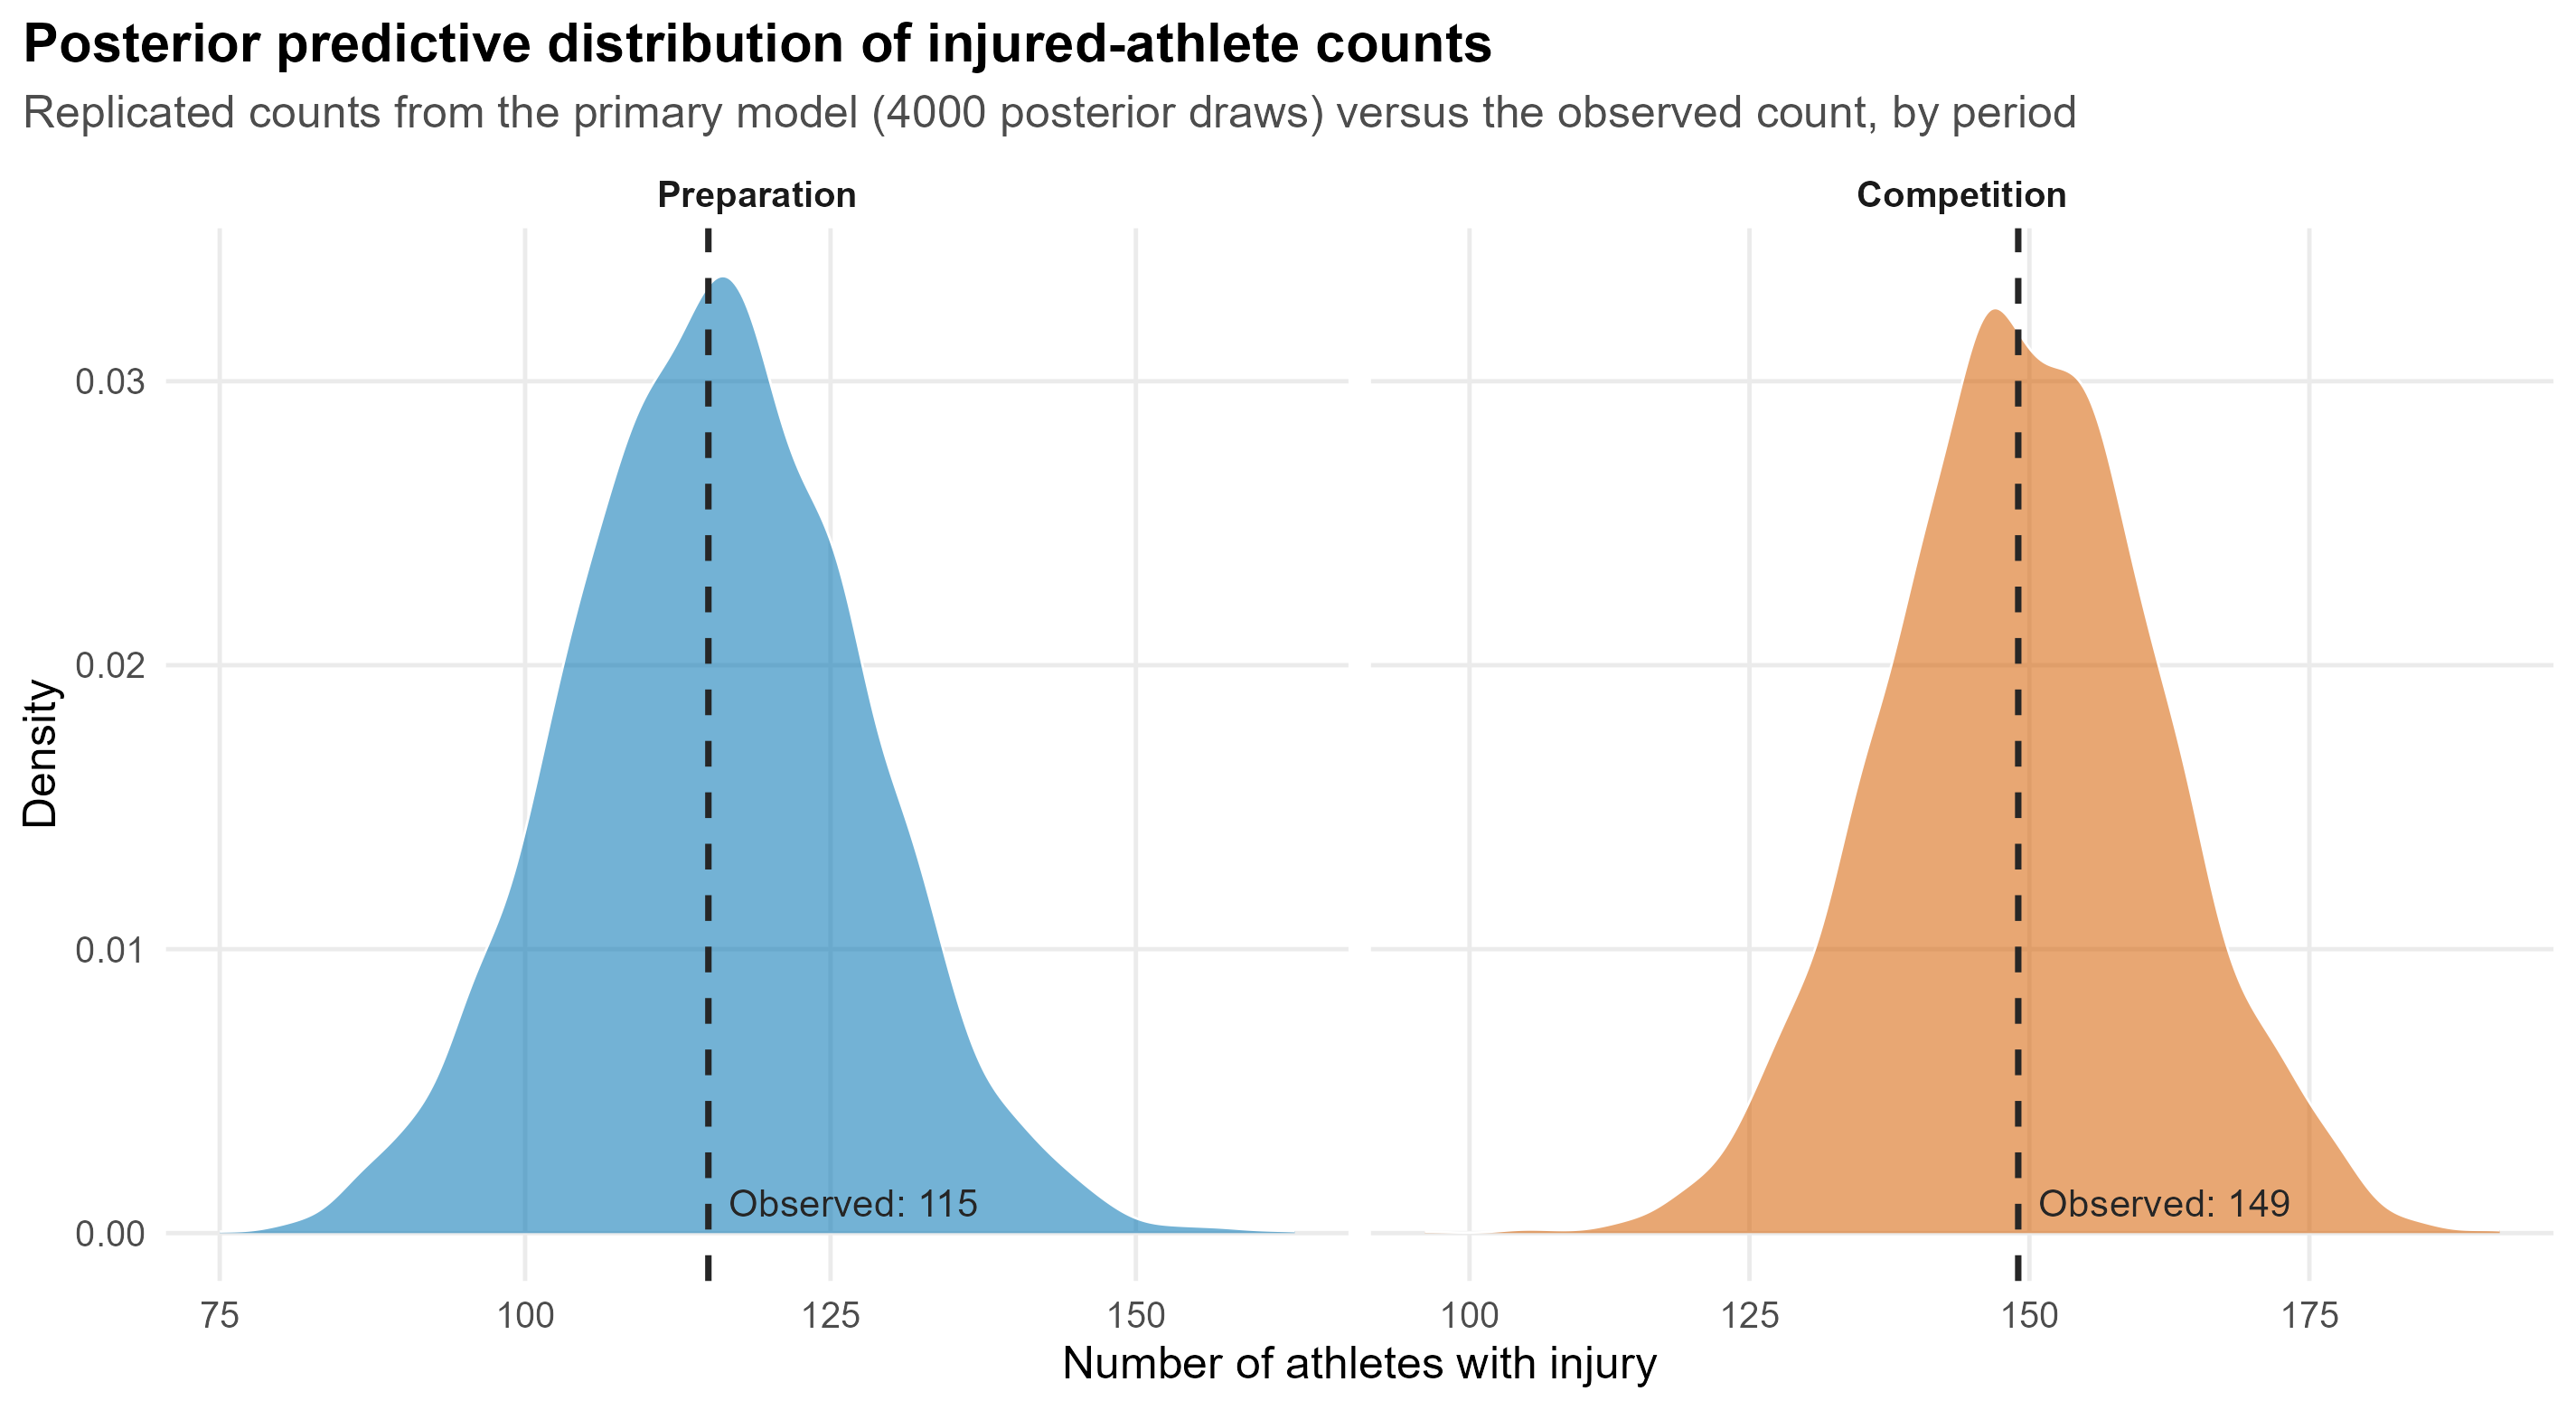
\includegraphics[width=0.85\textwidth]{fig_posterior_predictive.png}
\caption{Posterior predictive check: full posterior distribution of the model-replicated number of injured athletes (4000 posterior draws of the primary model), by period. Dashed vertical line: observed count.}
\label{fig:posterior-predictive}
\end{figure}

\begin{figure}[htbp]
\centering
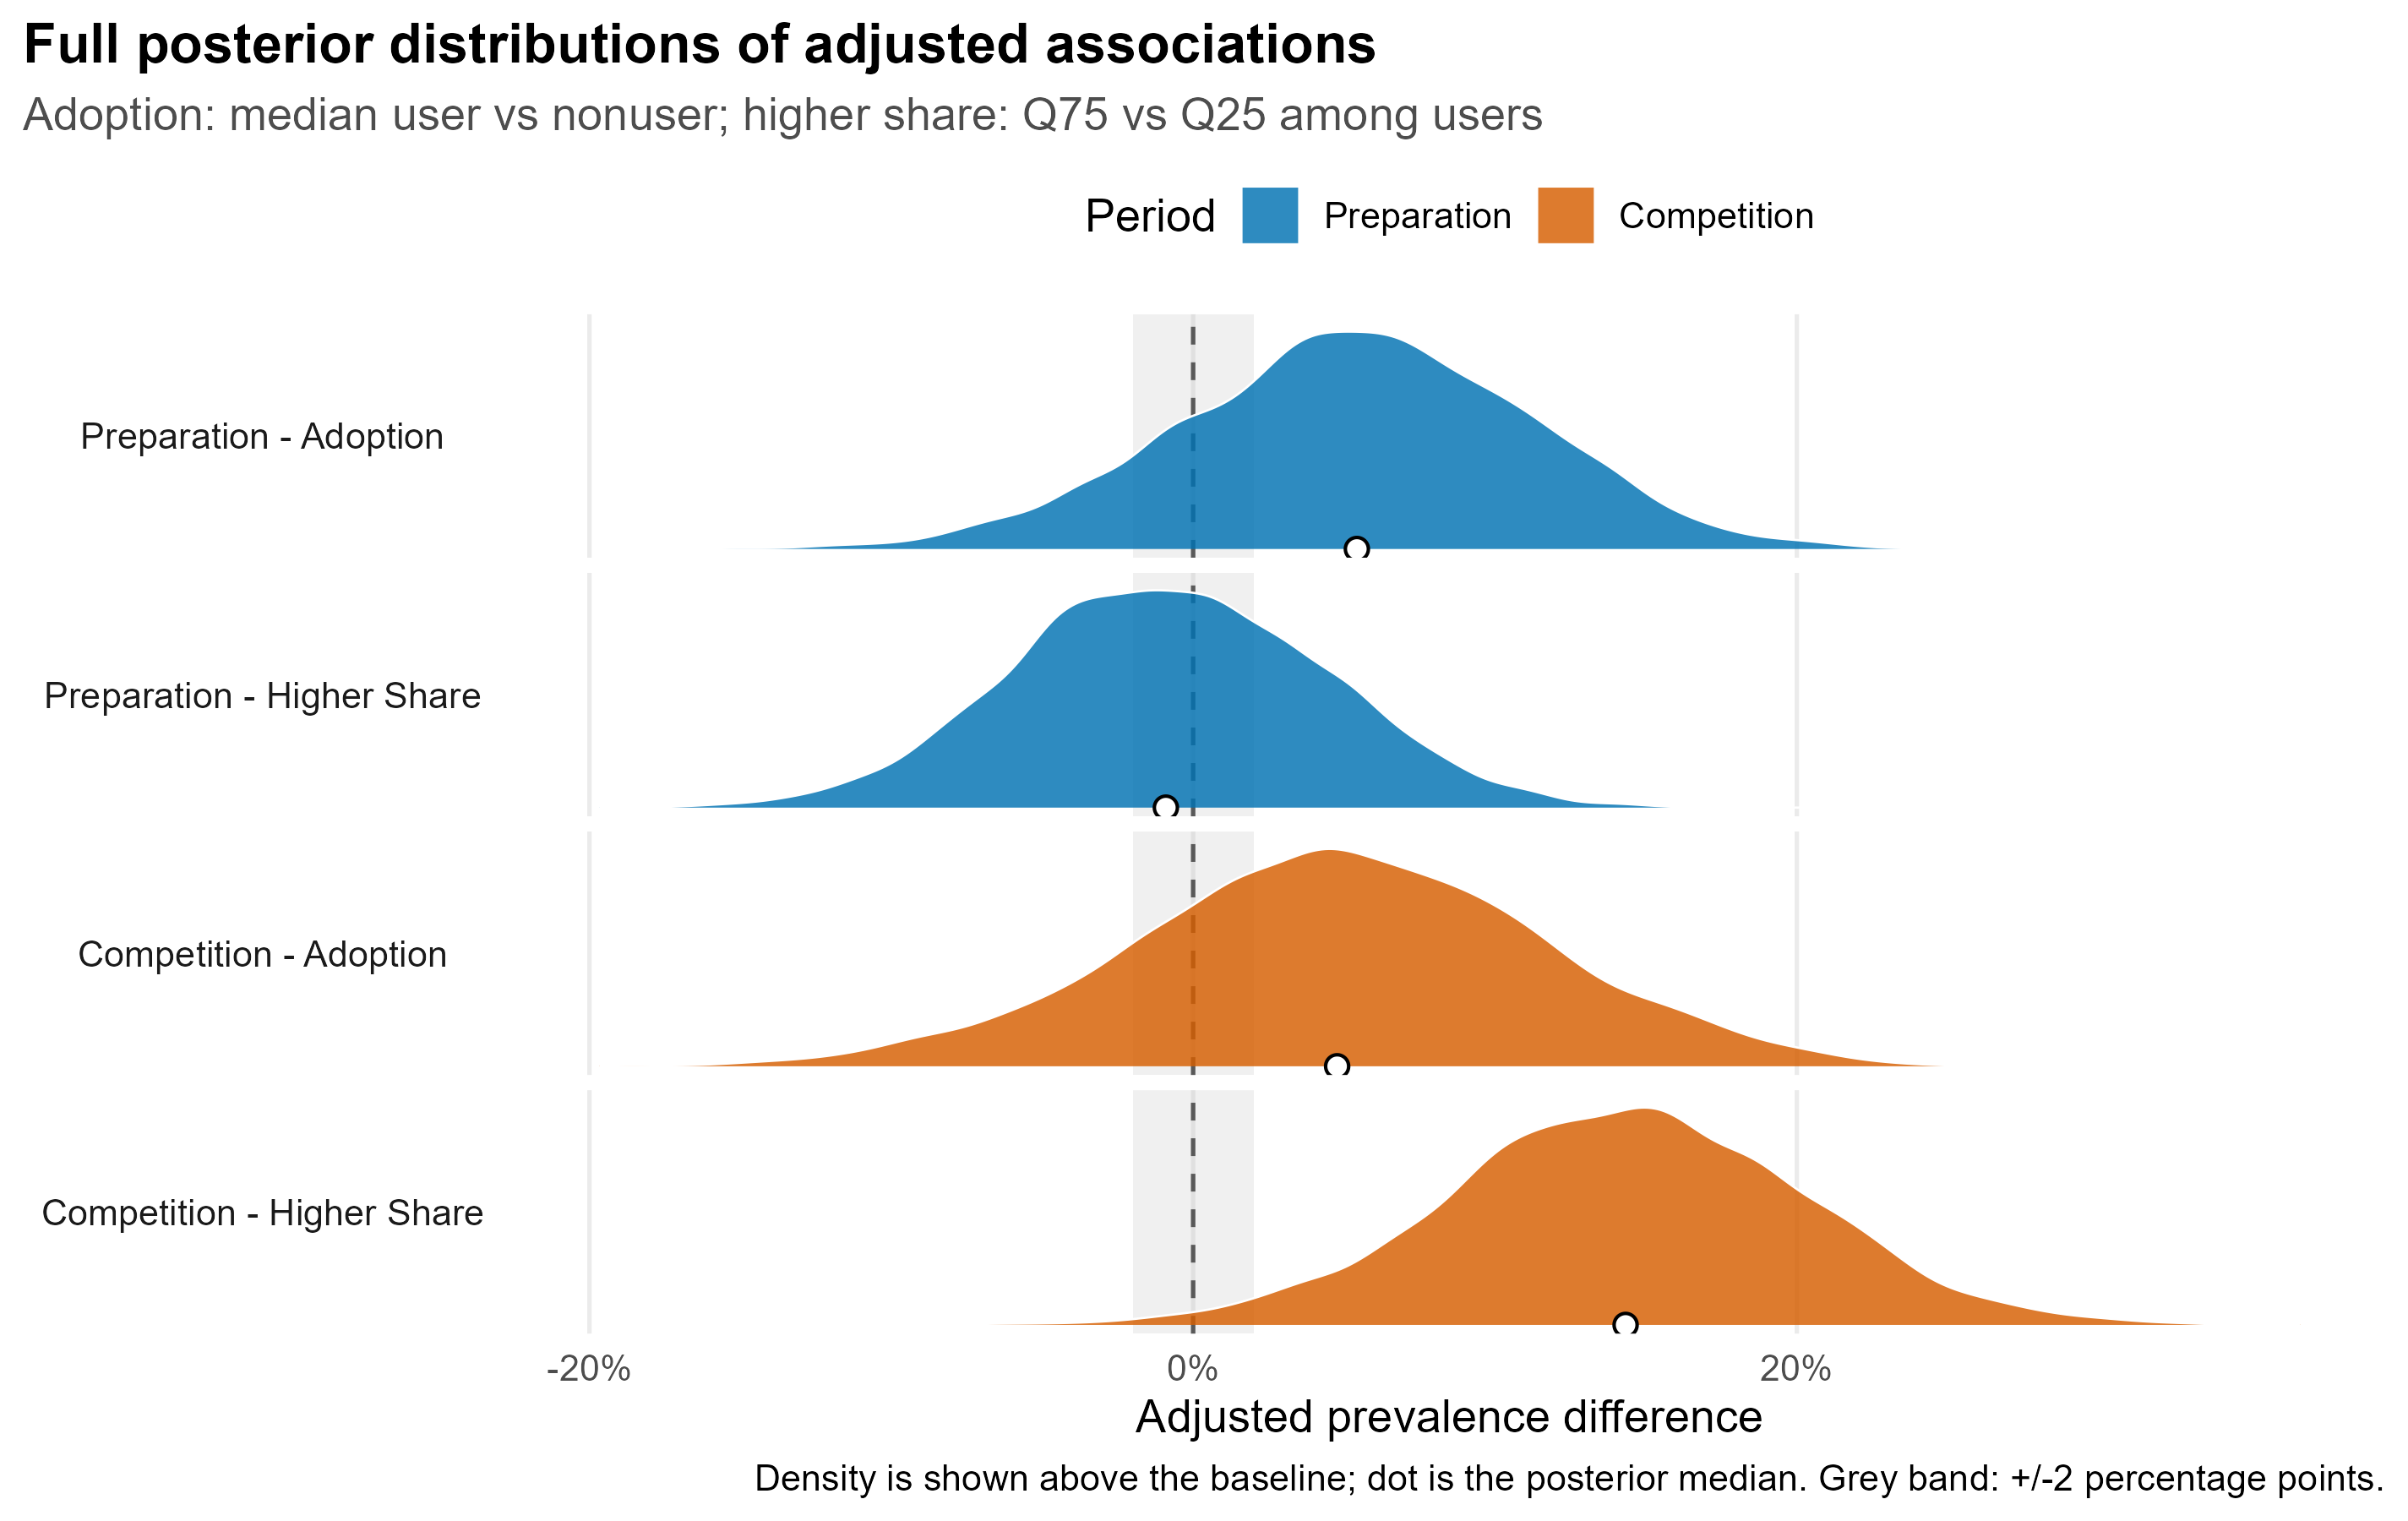
\includegraphics[width=0.8\textwidth]{fig_posterior_association_distributions.png}
\caption{Full posterior distributions of the adjusted prevalence-difference estimand for the adoption and dose contrasts, by period. Grey band: region of practical equivalence ($\pm$2 pp).}
\label{fig:posterior-associations}
\end{figure}

\begin{figure}[htbp]
\centering
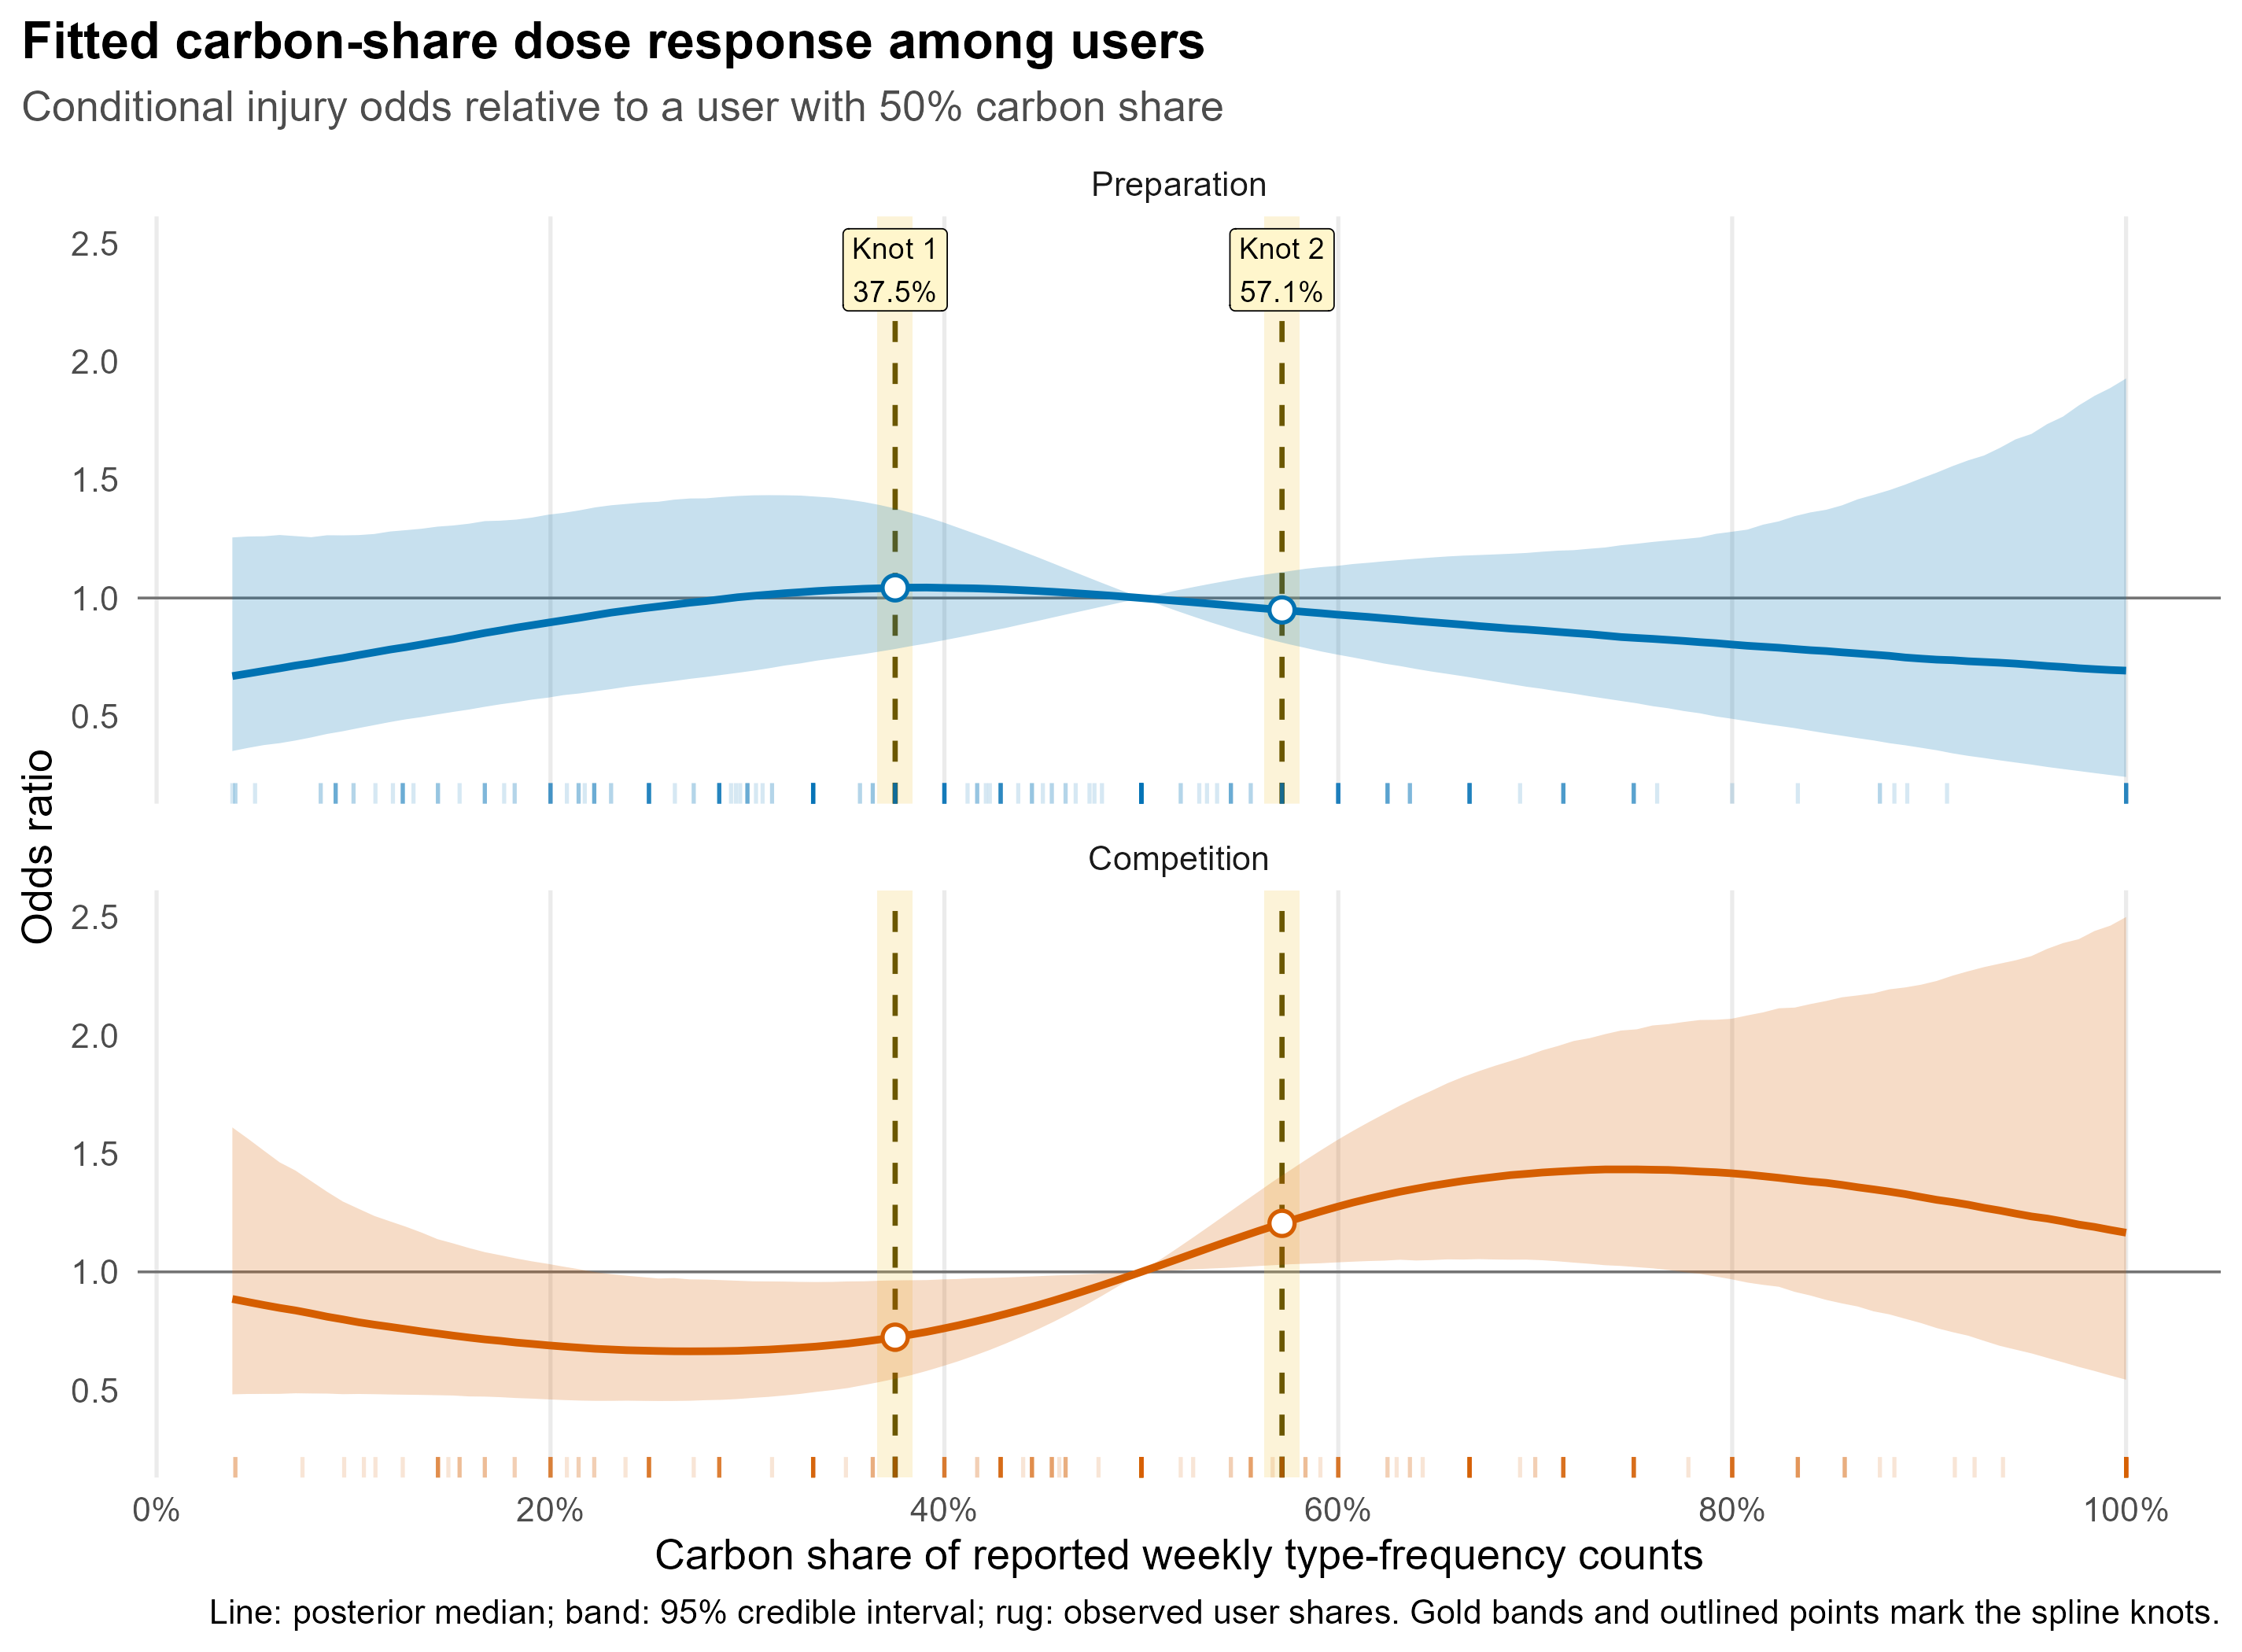
\includegraphics[width=0.85\textwidth]{fig_spline_dose_response.png}
\caption{Fitted carbon-share dose response among users. Curves are conditional injury odds relative to a user with 50\% carbon share; lines show posterior medians, bands 95\% credible intervals, and rugs observed user shares. Gold bands, labeled vertical lines, and outlined points mark the internal spline knots (37.5\% and 57.1\%).}
\label{fig:spline-dose-response}
\end{figure}

\begin{figure}[htbp]
\centering
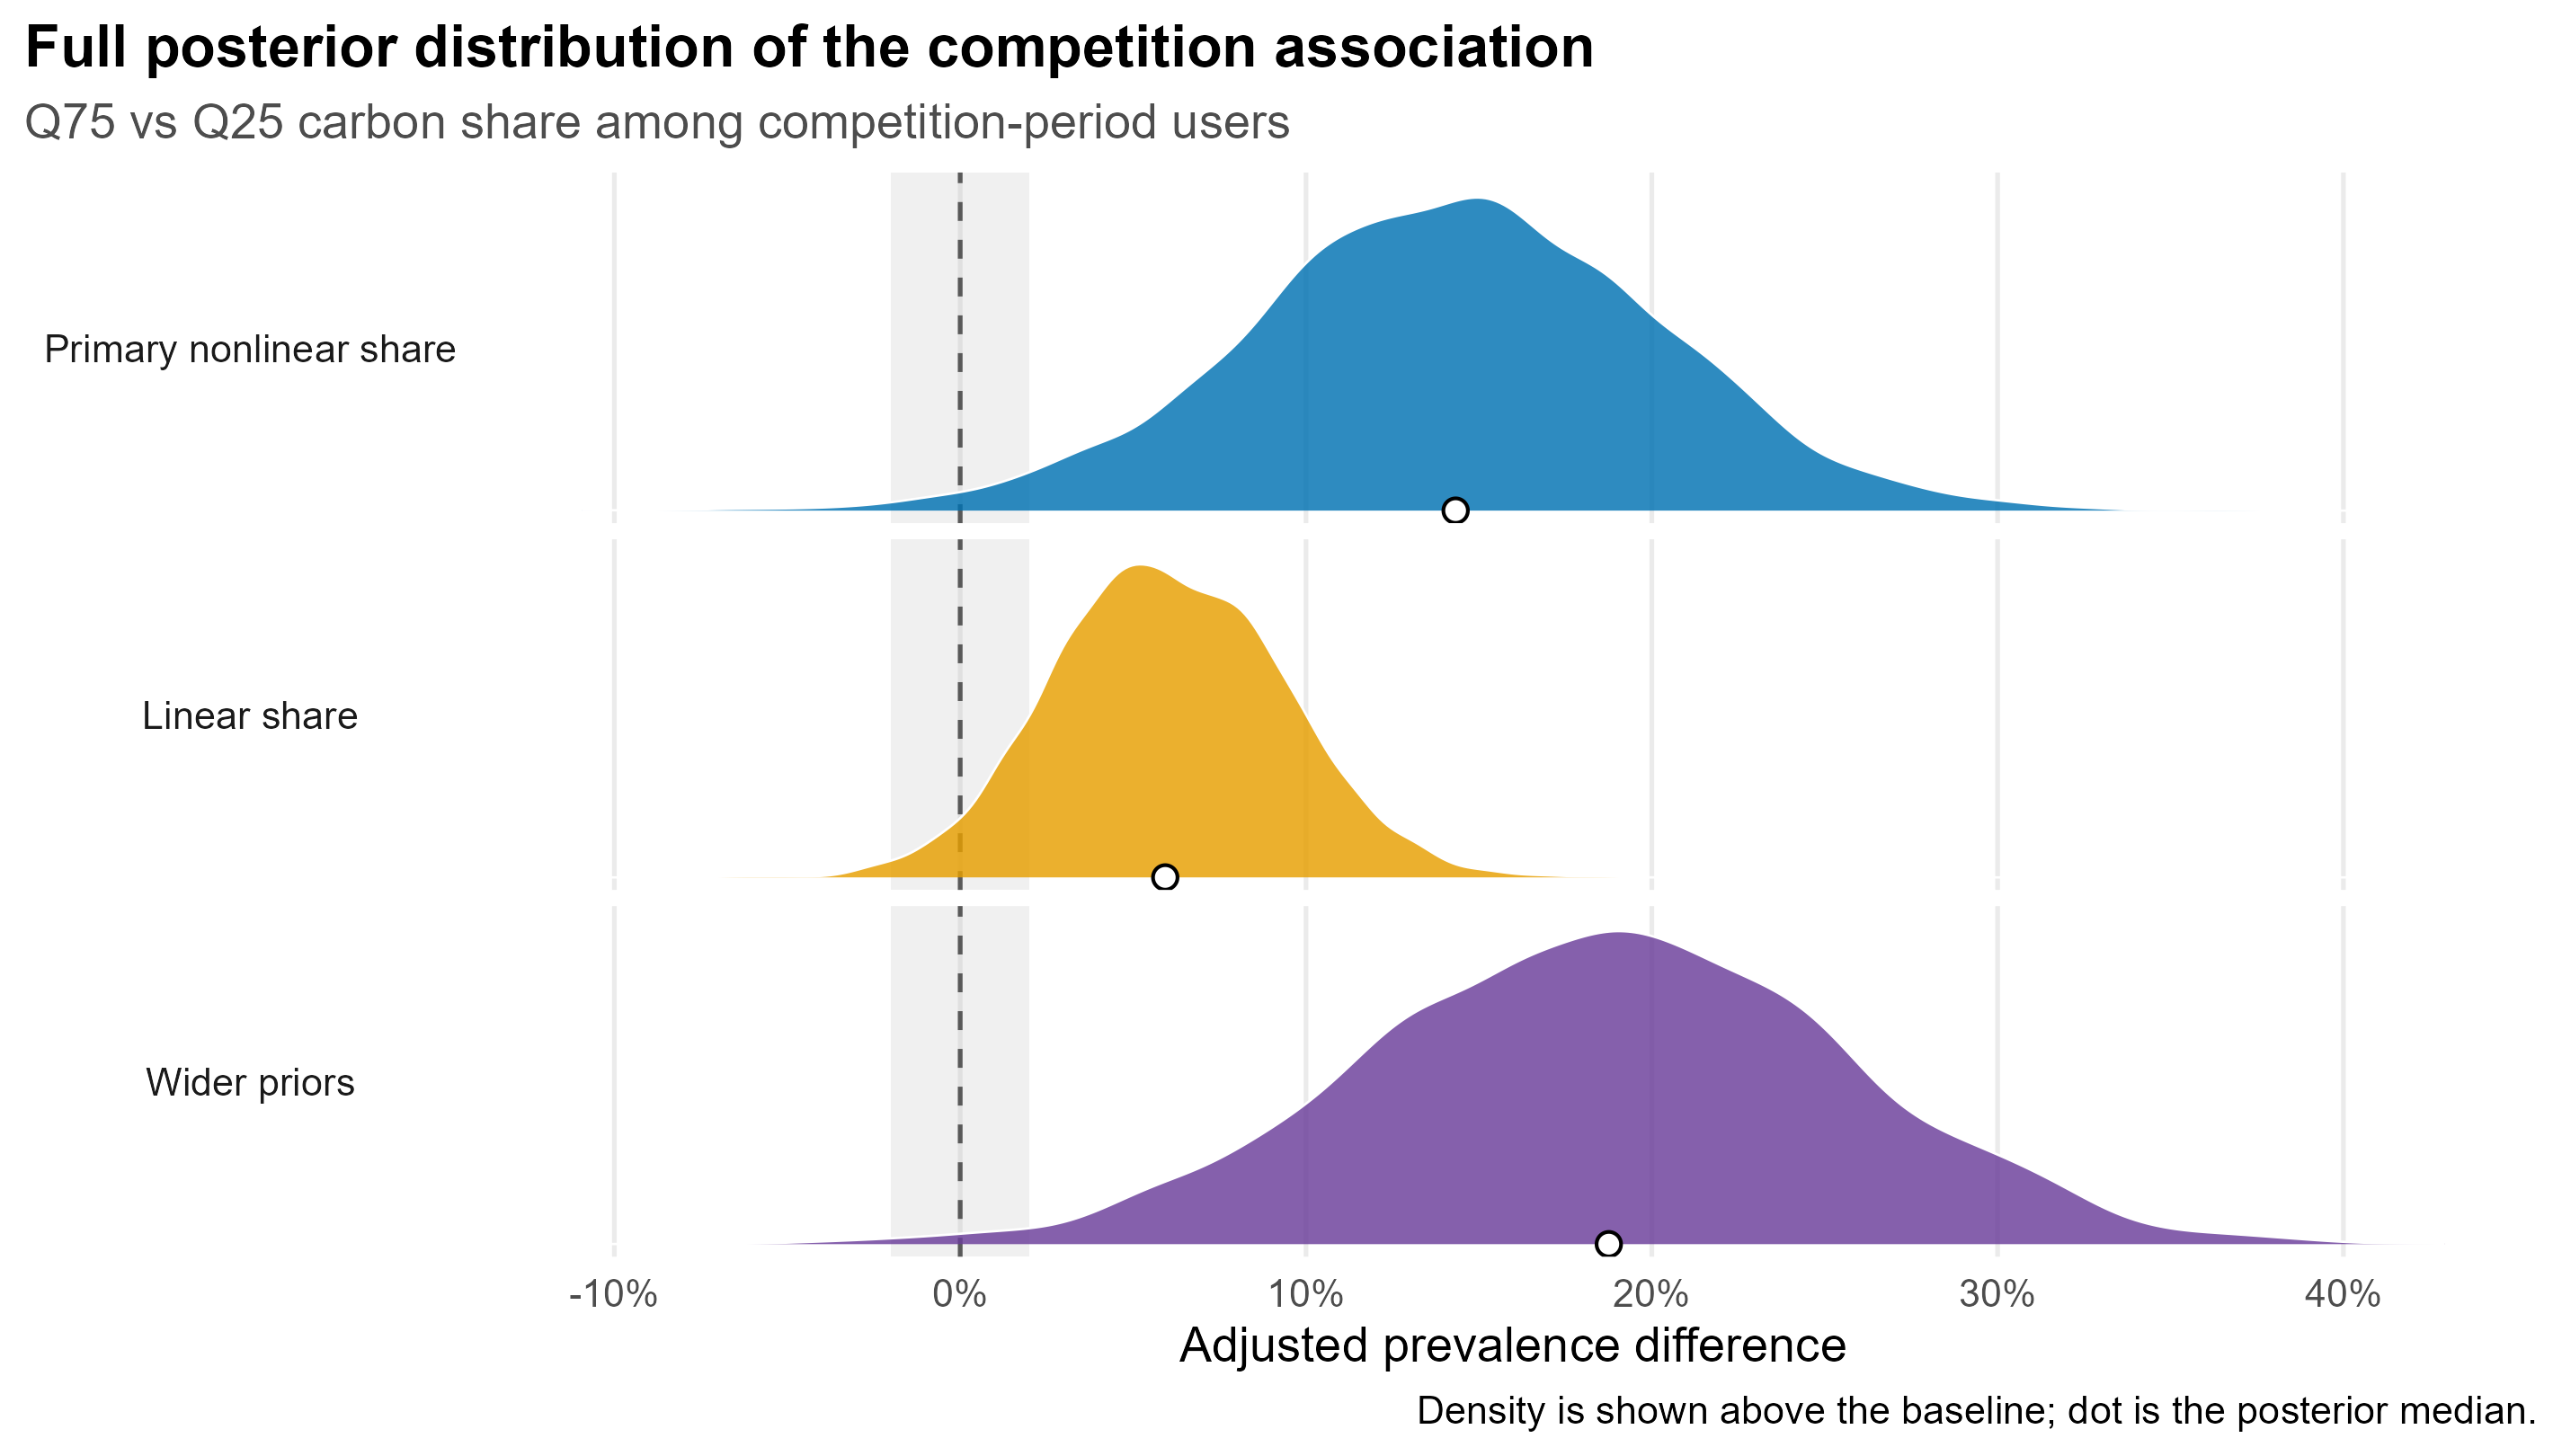
\includegraphics[width=0.8\textwidth]{fig_competition_dose_sensitivity.png}
\caption{Sensitivity analysis: full posterior distribution of the competition-period dose association (75th vs.\ 25th percentile carbon share among users) under the primary nonlinear specification, a linear share specification, and wider priors.}
\label{fig:competition-dose-sensitivity}
\end{figure}

\begin{figure}[htbp]
\centering
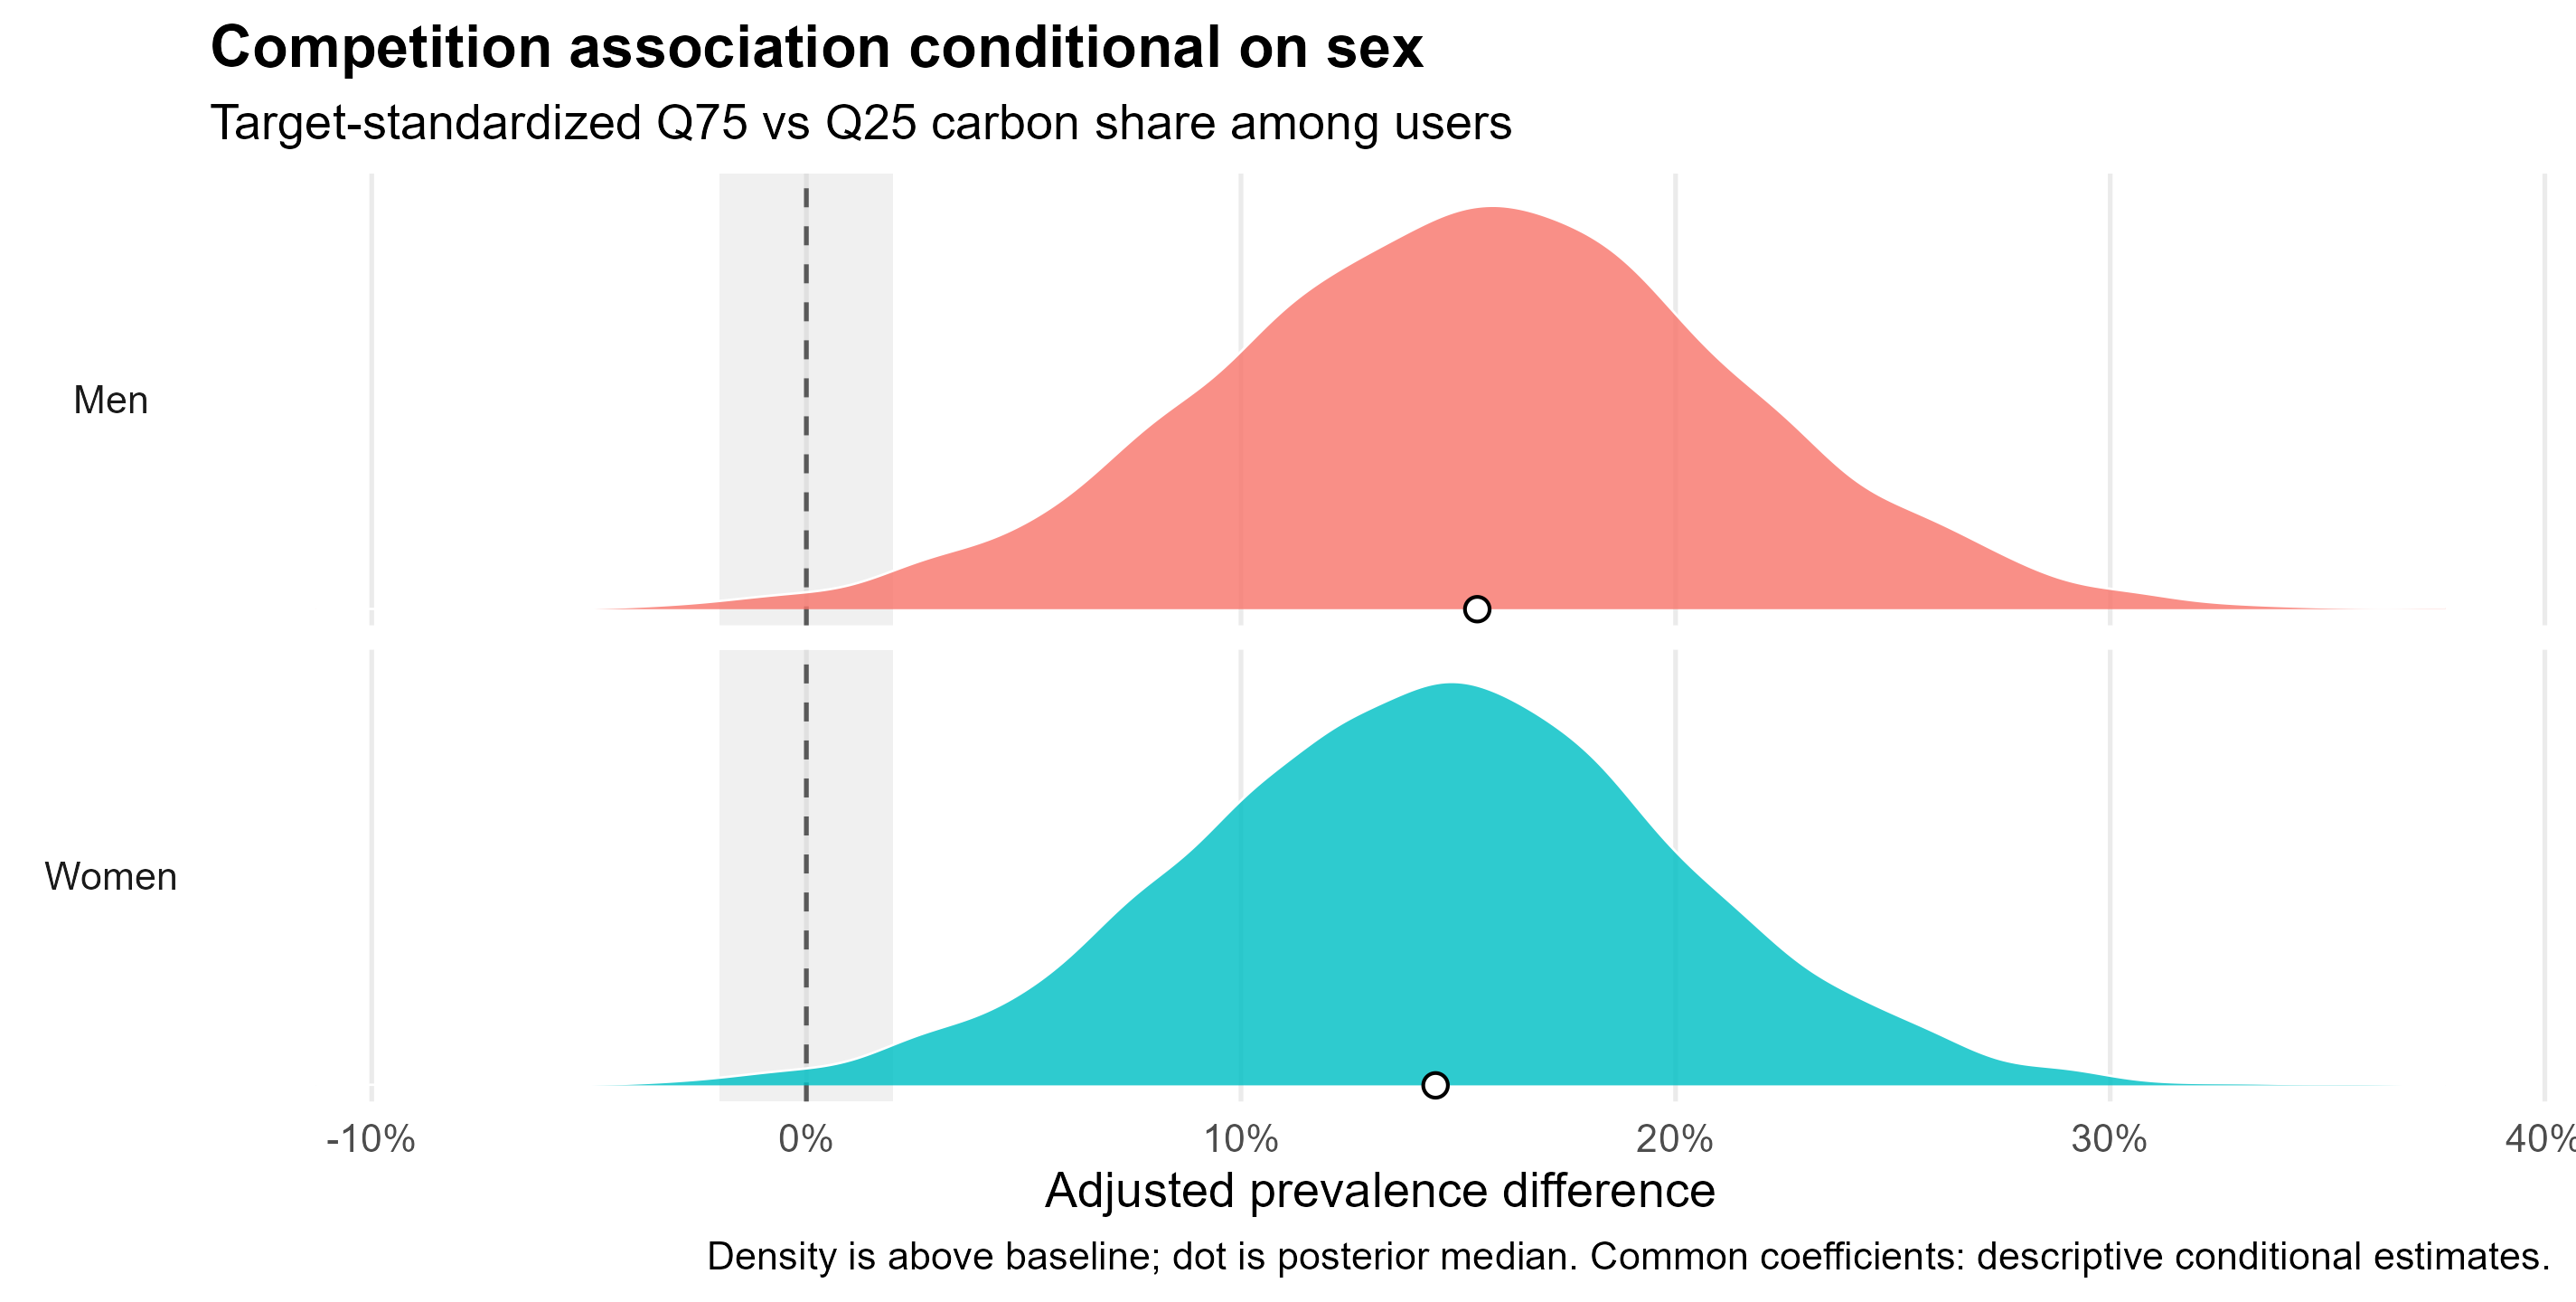
\includegraphics[width=0.75\textwidth]{fig_weighted_dose_by_sex.png}
\caption{Competition-period dose association, population-weighted and stratified by sex.}
\label{fig:weighted-dose-by-sex}
\end{figure}

\begin{figure}[htbp]
\centering
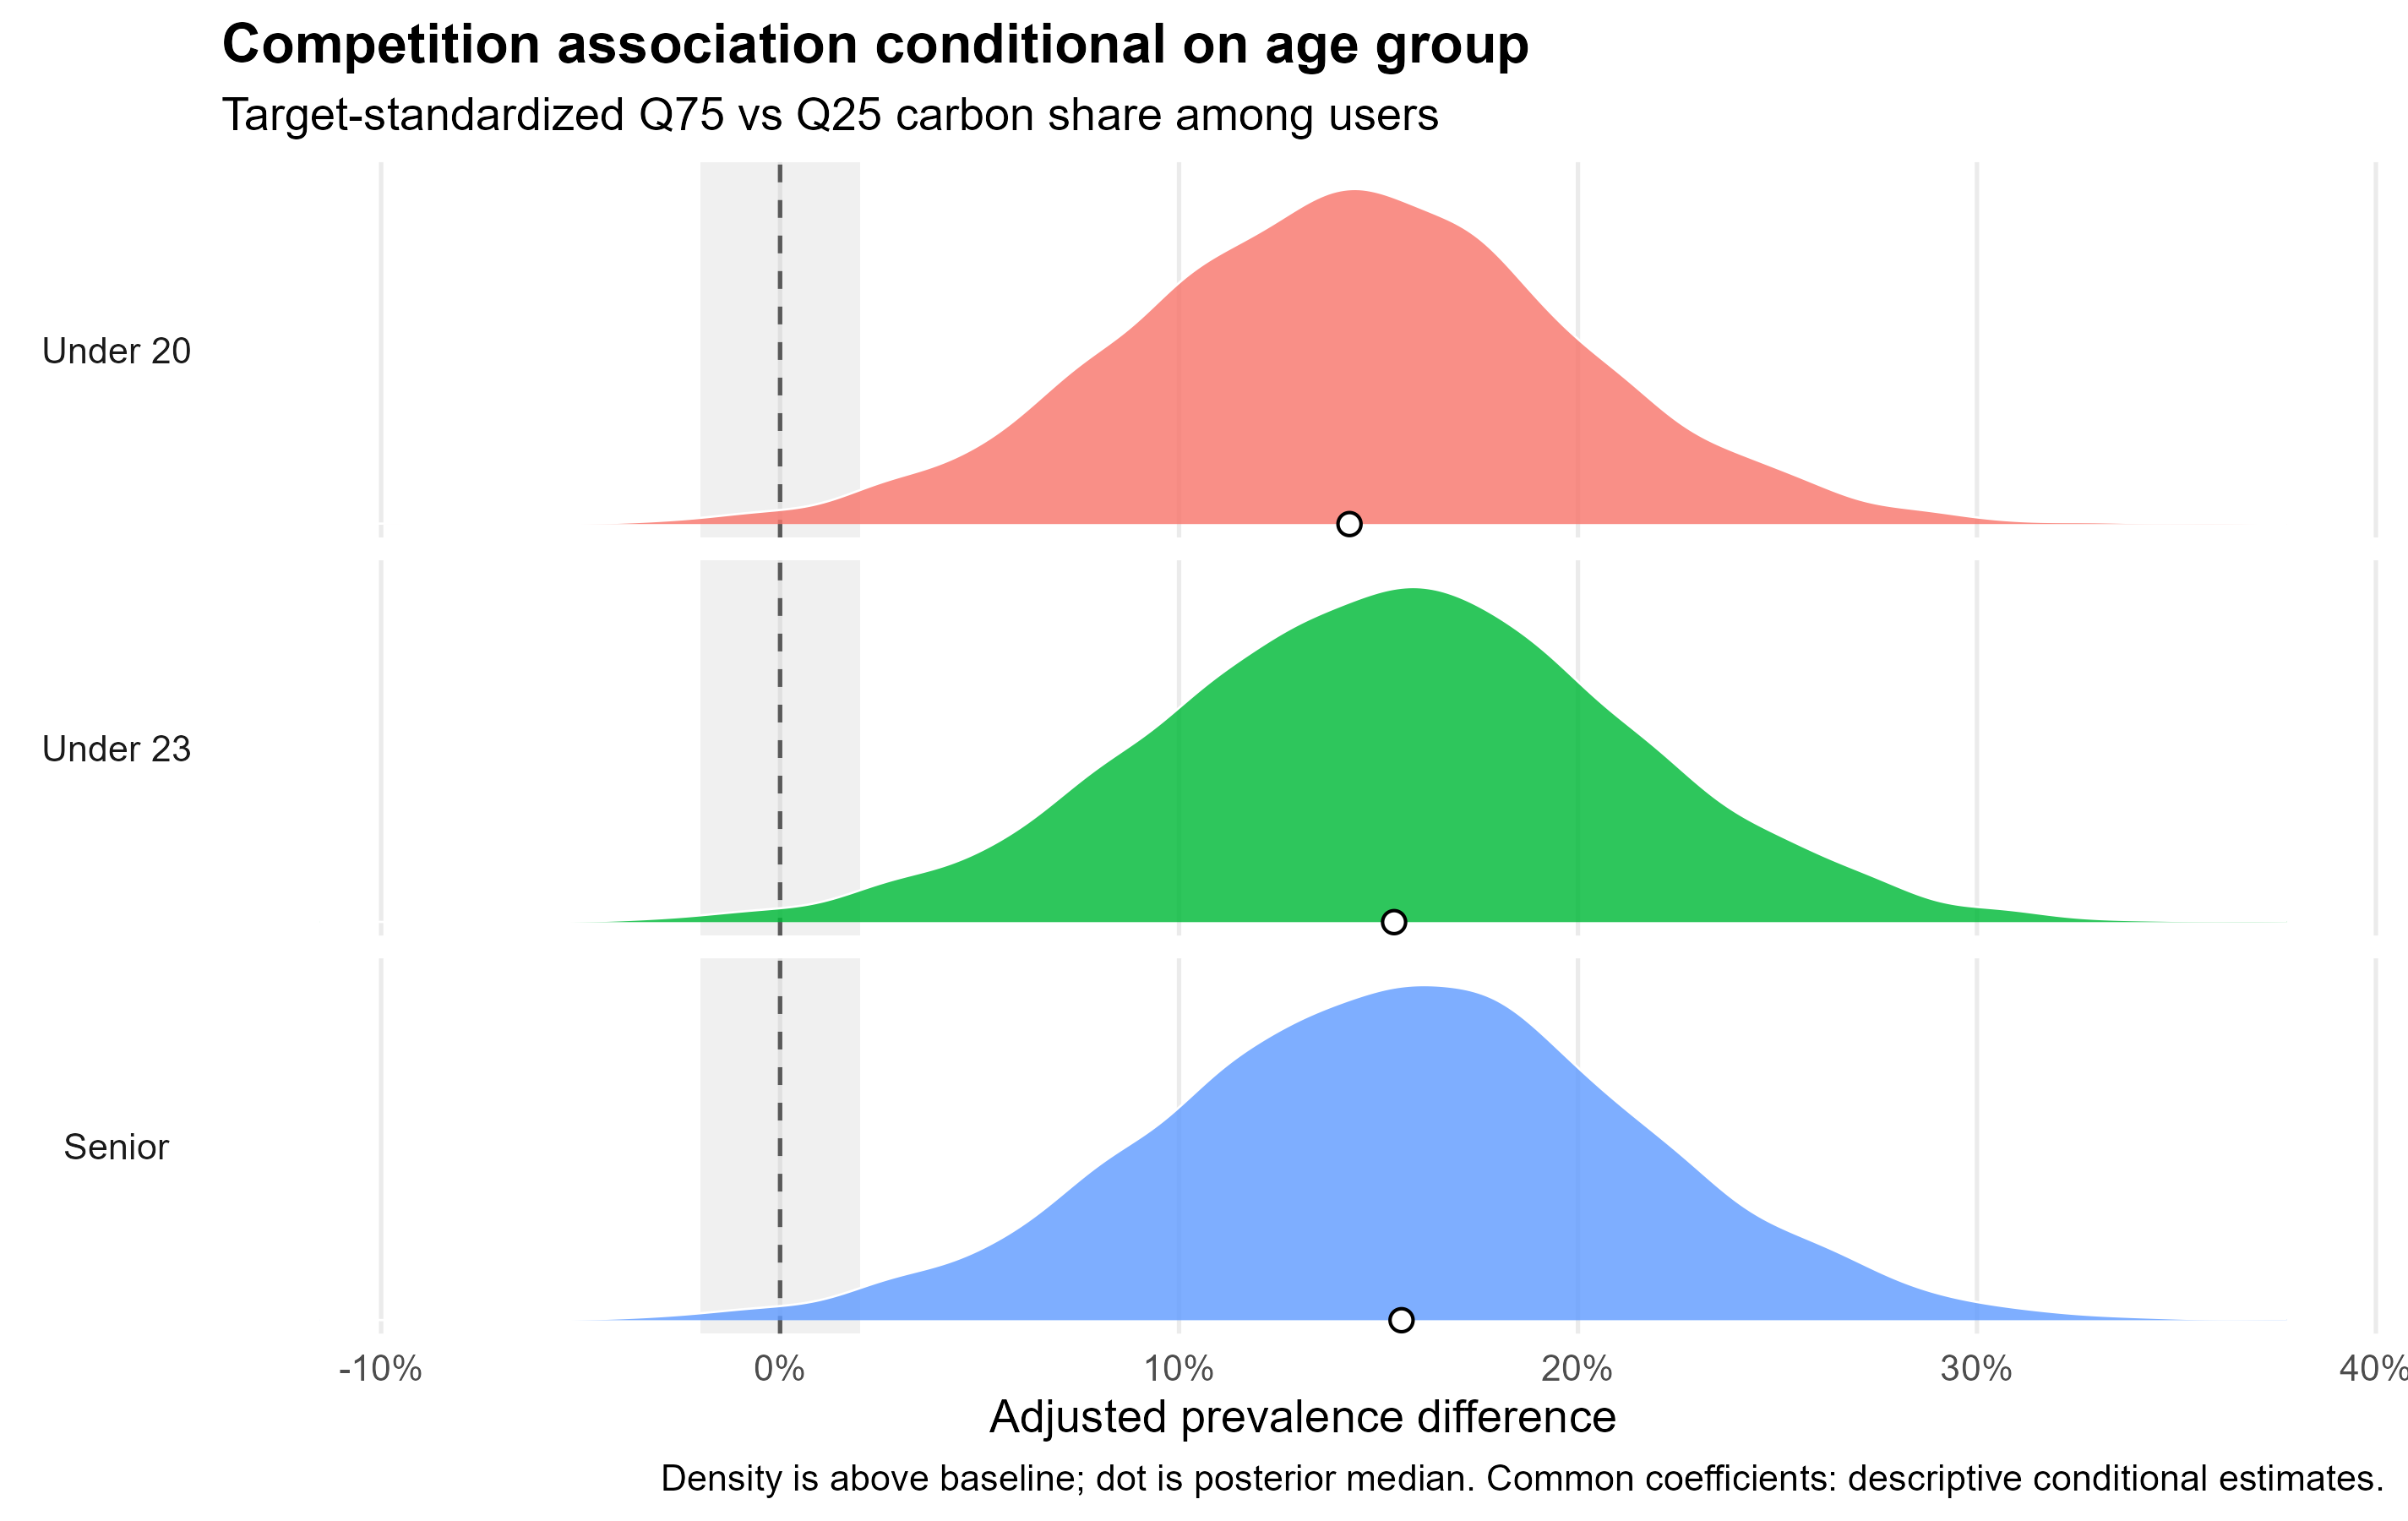
\includegraphics[width=0.75\textwidth]{fig_weighted_dose_by_age.png}
\caption{Competition-period dose association, population-weighted and stratified by age group.}
\label{fig:weighted-dose-by-age}
\end{figure}

\clearpage
\begingroup
\footnotesize
\begin{longtable}{L{3.3cm} L{1.9cm} C{1.7cm} C{1.7cm} C{1.6cm} C{1.6cm}}
\caption{Baseline characteristics of the balanced analysis cohort ($N=352$), by competition sex. Values are mean (SD), median [Q1, Q3], or n (\%). SMD is the standardized mean difference, women vs.\ men (Cohen's $d$ for continuous/ordinal rows, computed on log-odds for proportions); $|\text{SMD}| \geq 0.20$ is conventionally a small imbalance and $\geq 0.50$ a moderate one \citep{table1guidelines}. Population-weighted columns apply the age--sex poststratification weights of Section~\ref{sec:weighting} (Appendix Table~\ref{tab:weight-diagnostics}).}
\label{tab:table1}\\
\toprule
Characteristic & Statistic & Men ($n=194$) & Women ($n=158$) & SMD sample & SMD weighted\\
\midrule
\endfirsthead
\multicolumn{6}{l}{\textit{(continued)}}\\
\toprule
Characteristic & Statistic & Men ($n=194$) & Women ($n=158$) & SMD sample & SMD weighted\\
\midrule
\endhead
\midrule \multicolumn{6}{r}{\textit{(continued on next page)}}\\
\endfoot
\bottomrule
\endlastfoot
\multicolumn{6}{l}{\textbf{Demographics}}\\
Age, years & Mean (SD) & 21.3 (3.1) & 21.9 (3.1) & 0.198 & 0.137 \\
Age group: Under 20 & n (\%) & 71 (36.6) & 43 (27.2) & $-0.202$ & $-0.144$ \\
Age group: Under 23 & n (\%) & 63 (32.5) & 53 (33.5) & 0.023 & 0.060 \\
Age group: Senior & n (\%) & 60 (30.9) & 62 (39.2) & 0.175 & 0.093 \\
\multicolumn{6}{l}{\textbf{Anthropometrics}}\\
Height, cm & Mean (SD) & 180.6 (5.9) & 169.2 (6.8) & $-1.809$ & $-1.749$ \\
Weight, kg & Mean (SD) & 70.5 (7.8) & 57.8 (6.0) & $-1.831$ & $-1.847$ \\
\multicolumn{6}{l}{\textbf{Athletics history}}\\
Experience, years & Mean (SD) & 10.1 (4.4) & 11.0 (3.9) & 0.225 & 0.220 \\
\multicolumn{6}{l}{\textbf{Injury}}\\
Prior injury (previous 2 seasons) & n (\%) & 156 (80.4) & 111 (70.3) & $-0.237$ & $-0.250$ \\
Any current-season injury & n (\%) & 120 (61.9) & 84 (53.2) & $-0.177$ & $-0.210$ \\
Preparation-period injury & n (\%) & 69 (35.6) & 46 (29.1) & $-0.138$ & $-0.165$ \\
Competition-period injury & n (\%) & 88 (45.4) & 61 (38.6) & $-0.137$ & $-0.139$ \\
\multicolumn{6}{l}{\textbf{Carbon-plate insole exposure}}\\
Any preparation carbon use & n (\%) & 159 (82.0) & 128 (81.0) & $-0.024$ & $-0.041$ \\
Any competition carbon use & n (\%) & 173 (89.2) & 135 (85.4) & $-0.112$ & $-0.130$ \\
Preparation carbon share (among users) & Median [Q1,Q3] & 0.4 [0.2, 0.6] & 0.4 [0.3, 0.6] & 0.125 & 0.115 \\
Competition carbon share (among users) & Median [Q1,Q3] & 0.5 [0.3, 0.7] & 0.5 [0.4, 0.8] & 0.184 & 0.161 \\
\multicolumn{6}{l}{\textbf{Training frequency (period total)}}\\
Preparation total type-frequency & Median [Q1,Q3] & 8 [6, 11] & 8 [6, 13] & 0.098 & 0.069 \\
Competition total type-frequency & Median [Q1,Q3] & 7 [5, 10] & 7 [5, 11] & 0.121 & 0.106 \\
\multicolumn{6}{l}{\textbf{Discipline}}\\
Sprint & n (\%) & 64 (33.0) & 43 (27.2) & $-0.126$ & $-0.122$ \\
Middle distance & n (\%) & 38 (19.6) & 31 (19.6) & 0.001 & 0.015 \\
Long distance & n (\%) & 36 (18.6) & 23 (14.6) & $-0.108$ & $-0.064$ \\
Hurdles & n (\%) & 51 (26.3) & 45 (28.5) & 0.049 & 0.023 \\
Horizontal jumps & n (\%) & 18 (9.3) & 26 (16.5) & 0.216 & 0.183 \\
Pole vault & n (\%) & 10 (5.2) & 9 (5.7) & 0.024 & 0.001 \\
Combined events & n (\%) & 16 (8.2) & 25 (15.8) & 0.234 & 0.195 \\
\end{longtable}
\endgroup

\begin{table}[htbp]
\centering
\caption{Sample flow from survey respondents to the balanced analysis cohort.}
\label{tab:sample-flow}
\begin{tabular}{lr}
\toprule
Stage & n \\
\midrule
Consented, eligible, complete survey & 355 \\
\quad Excluded: incomplete injury timing & $-1$ \\
\quad Excluded: zero total eligible frequency in a period & $-2$ \\
Balanced analysis cohort (athletes) & 352 \\
Athlete-period records (preparation + competition) & 704 \\
\midrule
Preparation-period injuries & 115 \\
Competition-period injuries & 149 \\
\bottomrule
\end{tabular}
\end{table}

\begin{table}[htbp]
\centering
\caption{Mean reported carbon share of training-type frequency, overall and by sex and age group. Carbon share is defined in Section~\ref{sec:exposure} and includes non-users (share $=0$).}
\label{tab:descriptive-carbon}
\begin{tabular}{llrrr}
\toprule
Stratum & Level & n & Preparation, mean share & Competition, mean share \\
\midrule
Overall & Overall & 352 & 0.357 & 0.477 \\
Sex & Men & 194 & 0.349 & 0.468 \\
 & Women & 158 & 0.366 & 0.488 \\
Age group & Under 20 & 114 & 0.365 & 0.453 \\
 & Under 23 & 116 & 0.379 & 0.489 \\
 & Senior & 122 & 0.328 & 0.488 \\
\bottomrule
\end{tabular}
\end{table}

\begingroup
\footnotesize
\begin{longtable}{L{3.3cm} C{0.7cm} C{1.15cm} C{0.95cm} C{1.15cm} C{1.15cm} C{1.05cm} C{1.15cm} C{1.05cm} C{1.05cm}}
\caption{Characteristics and injury prevalence by specialty group. Groups collapse the seven athletics disciplines (Appendix Table~\ref{tab:discipline-support}) into four physiologically motivated categories: Sprint/hurdles (sprint or hurdles), Endurance (middle or long distance), Jumps (horizontal jumps or pole vault), and Combined events. Because disciplines and, consequently, groups are multi-select, 26 of 352 athletes belong to more than one group.}
\label{tab:specialty-group}\\
\toprule
& $n$ & Age, y & Women, \% & Height, cm & Weight, kg & Exp., y & Prior inj., \% & Any inj., \% & Comp.\ inj., \% \\
\midrule
\endfirsthead
\multicolumn{10}{l}{\textit{(continued)}}\\
\toprule
& $n$ & Age, y & Women, \% & Height, cm & Weight, kg & Exp., y & Prior inj., \% & Any inj., \% & Comp.\ inj., \% \\
\midrule
\endhead
\midrule \multicolumn{10}{r}{\textit{(continued on next page)}}\\
\endfoot
\bottomrule
\endlastfoot
Sprint/hurdles & 169 & 21.4 (3.0) & 42.6 & 175.8 (8.7) & 66.9 (9.3) & 10.0 (3.9) & 75.7 & 60.9 & 44.4 \\
Endurance & 109 & 21.6 (3.2) & 42.2 & 174.0 (8.2) & 59.6 (7.9) & 10.3 (4.3) & 67.9 & 44.0 & 30.3 \\
Jumps & 62 & 22.2 (3.5) & 54.8 & 175.6 (9.0) & 65.8 (9.6) & 11.5 (4.6) & 83.9 & 64.5 & 51.6 \\
Combined events & 41 & 22.0 (3.0) & 61.0 & 176.6 (7.4) & 67.8 (8.3) & 11.9 (4.4) & 82.9 & 70.7 & 48.8 \\
\end{longtable}
\endgroup

\begin{table}[htbp]
\centering
\footnotesize
\caption{Carbon-plate insole use and training-type frequency by specialty group (grouping as in Table~\ref{tab:specialty-group}).}
\label{tab:specialty-group-carbon}
\begin{tabular}{lcccc}
\toprule
Specialty group & Prep.\ carbon share & Comp.\ carbon share & Prep.\ total freq., Mdn & Comp.\ total freq., Mdn \\
\midrule
Sprint/hurdles & 0.39 & 0.56 & 8 & 7 \\
Endurance & 0.31 & 0.34 & 10 & 9 \\
Jumps & 0.33 & 0.47 & 6 & 5 \\
Combined events & 0.41 & 0.52 & 9 & 9 \\
\bottomrule
\end{tabular}
\end{table}

\begin{table}[htbp]
\centering
\footnotesize
\caption{Anatomical location of reported injuries (259 injuries among 204 injured athletes; multi-select item, so location counts sum to more than 259).}
\label{tab:injury-location}
\begin{tabular}{lrrr}
\toprule
Location & Injuries, $n$ & \% of injuries & \% of injured athletes ($n=204$) \\
\midrule
Thigh (anterior or posterior) & 97 & 37.5 & 39.2 \\
Lower leg (anterior or posterior) & 65 & 25.1 & 27.9 \\
Foot (anterior or posterior) & 50 & 19.3 & 22.1 \\
Ankle (medial or lateral) & 36 & 13.9 & 15.2 \\
Groin & 26 & 10.0 & 12.3 \\
Hip & 14 & 5.4 & 6.9 \\
Head, upper limb, or trunk & 11 & 4.2 & 5.4 \\
\bottomrule
\end{tabular}
\end{table}

\begin{table}[htbp]
\centering
\footnotesize
\caption{Type of reported lower-limb injuries. The type item was asked only for injuries localized to the hip, groin, thigh, lower leg, ankle, or foot (248 of 259 injuries; the questionnaire ended after the location item for the 11 head/upper-limb/trunk injuries); multi-select item, so counts sum to more than 248.}
\label{tab:injury-type}
\begin{tabular}{lrrr}
\toprule
Type & Injuries, $n$ & \% of lower-limb injuries & \% of injured athletes ($n=204$) \\
\midrule
Tendinopathy & 71 & 28.6 & 29.9 \\
Bone stress injury or stress fracture & 65 & 26.2 & 25.0 \\
Muscle strain & 55 & 22.2 & 26.5 \\
Other & 39 & 15.7 & 16.7 \\
Ligament injury & 18 & 7.3 & 8.8 \\
Plantar fasciopathy & 16 & 6.5 & 7.8 \\
Joint sprain & 14 & 5.6 & 6.9 \\
Tendon rupture & 10 & 4.0 & 3.9 \\
\bottomrule
\end{tabular}
\end{table}

\begin{table}[htbp]
\centering
\footnotesize
\caption{Anatomical location of the three leading injury types (\% of injuries of that type; multi-select, so rows sum to more than 100\%). Location categories with 0\% in all three rows (hip, groin, head/upper limb/trunk) are omitted.}
\label{tab:injury-type-by-location}
\begin{tabular}{lrrrr}
\toprule
Type ($n$ injuries) & Thigh & Lower leg & Ankle & Foot \\
\midrule
Tendinopathy (71) & 22.5 & 33.8 & 22.5 & 35.2 \\
Bone stress injury/stress fracture (65) & 58.5 & 26.2 & 7.7 & 15.4 \\
Muscle strain (55) & 74.5 & 27.3 & 3.6 & 0.0 \\
\bottomrule
\end{tabular}
\end{table}

\begin{table}[htbp]
\centering
\caption{Primary adjusted associations between carbon-plate insole exposure and injury prevalence, by period and contrast. Adjusted prevalence difference and ratio are posterior-standardized (Section~\ref{sec:estimands}); credible intervals are 95\% equal-tailed. Adoption compares the median-share user with a non-user; dose compares the 75th with the 25th percentile of share among users.}
\label{tab:primary-associations}
\begin{tabular}{llrrr}
\toprule
Period & Contrast & Difference, pp (95\% CrI) & Ratio (95\% CrI) & P(positive) \\
\midrule
Preparation & Adoption & 5.4 ($-6.3$ to $16.2$) & 1.21 (0.84 to 1.74) & 82.0\% \\
Preparation & Dose & $-0.8$ ($-10.6$ to $9.1$) & 0.99 (0.73 to 1.30) & 43.8\% \\
Competition & Adoption & 4.8 ($-8.7$ to $17.7$) & 1.16 (0.82 to 1.65) & 77.1\% \\
Competition & Dose & \textbf{14.3 (2.7 to 25.8)} & \textbf{1.41 (1.06 to 1.86)} & \textbf{99.0\%} \\
\bottomrule
\end{tabular}
\end{table}

\begin{table}[htbp]
\centering
\caption{Sensitivity of the competition-period dose association (75th vs.\ 25th percentile share among users) to model specification.}
\label{tab:sensitivity}
\begin{tabular}{lrr}
\toprule
Model & Difference, pp (95\% CrI) & P(positive) \\
\midrule
Primary (nonlinear spline share) & 14.3 (2.7 to 25.8) & 99.0\% \\
Linear share & 6.0 ($-0.3$ to $12.6$) & 96.9\% \\
Wider priors & 18.7 (5.2 to 31.9) & 99.5\% \\
\bottomrule
\end{tabular}
\end{table}

\clearpage


\section{Discussion}
\label{sec:discussion}
\subsection{Key results}
\label{sec:discussion-key}
This national, two-phase-recruited sample of competitive Italian athletics athletes shows carbon-plated spikes established as the prevailing training equipment: a mean 35.7\% of preparation-period and 47.7\% of competition-period training-type frequency, with adoption above 80\% in both periods and a consistent pattern across sex and age-group strata. Adoption was not clearly associated with injury prevalence in either period. Among competition-period users, the primary nonlinear share model showed higher adjusted injury prevalence at higher share, but the matched linear comparison showed that this association was not unique to the relative scale: an increase from 37.3\% to 61.4\% share (24.1 percentage points) corresponded to a 7.9-pp risk difference (95\% CrI 1.4 to 14.4; $P_{\mathrm{dir}}=99.0\%$), while an increase from 2.83 to 6.19 units of the summed ordinal carbon-frequency score (3.36 units, not unique sessions) corresponded to 8.3 pp (95\% CrI 1.6 to 15.9; $P_{\mathrm{dir}}=99.2\%$). Both preparation estimates remained uncertain. The adapted OSTRC-H2 items added an athlete-centered burden estimate beyond injury counts: median severity was 75 of 100 and was highest among athletes reporting injuries in both periods. A further original descriptive finding reinforces this pattern: among the 248 lower-limb injuries with a recorded type, tendinopathy (28.6\%) and bone stress injury or stress fracture (26.2\%) were the two leading injury types, together exceeding muscle strain (22.2\%)--a distribution markedly different from general athletics injury surveillance, where muscle injury typically predominates \citep{edouard2020injury}. Cross-tabulating type against location refines this further: tendinopathy was disproportionately concentrated at the foot, lower leg, and ankle relative to the injury sample as a whole, a distal pattern that lines up with the Achilles- and forefoot-tendon loading flagged by the biomechanical literature on carbon-plate use (Section~\ref{sec:discussion-comparison}); bone stress injury, by contrast, was thigh-dominant like the sample overall, so its elevated frequency in this cohort is a genuine finding but is not, on the present data, specifically localized to the foot or ankle.

\subsection{Interpretation}
\label{sec:discussion-interpretation}
The distinction between adoption and amount of use remains central: the association tracked greater competition-period exposure among users, not simply adoption. The exposure-scale comparison, however, changes the mechanistic interpretation. Similar standardized estimates for share and absolute frequency mean that these data cannot identify whether relative allocation to carbon footwear or cumulative carbon-use frequency is the more relevant quantity. The two measures are mathematically related and were therefore fitted separately; adjustment for period-matched total training frequency makes each coefficient conditional on reported training volume but does not turn their descriptive comparison into causal separation. The result is compatible with a cumulative-load mechanism in which greater exposure to altered longitudinal bending stiffness changes ankle and plantarflexor loading \citep{gerlach2025aft,willwacher2016stiffness}, but it is also compatible with unmeasured competition-period intensity, footwear allocation, or reverse causation.

The primary HSGP curve, its linear sensitivity analysis, and the matched standardized models agree on the positive direction of the competition association, at a magnitude estimated in the 6--15 pp range across specifications. The empirical P75-versus-P25 estimate is a summary of one continuously estimated dose--response curve, not evidence for a threshold or for share as the clinically privileged scale. Likewise, the exact 25\%, 50\%, and 75\% values shown on the profile-specific curve are interpretive anchors on that same curve: no athlete groups were formed at those values, and the model did not estimate change-points at 25\%, 50\%, or 75\%. The profile-specific outputs add clinical interpretability by expressing fitted associations as absolute injury probabilities while holding measured characteristics constant; the same models can generate predictions for other specified profiles, and validating them as individual risk calculators is a task for future, externally validated work. The appropriately scoped conclusion is that greater reported competition-period carbon exposure among users was associated with greater adjusted injury prevalence on both examined scales--a population-level signal worth acting on through monitoring, even though its precise magnitude is not yet settled. Prospective measurement of unique carbon-shoe sessions, duration, intensity, and temporal order is needed to distinguish relative from cumulative exposure and to assess causality.

The OSTRC findings also show why injury burden should not be reduced to absence or complete cessation from sport. Time-loss-only systems can underestimate overuse problems that impair training, performance, or symptoms while athletes continue to participate \citep{clarsen2013ostrc,clarsen2020ostrc}. Direct athlete reporting therefore complements injury counts and time loss with consequences that matter to the athlete. In this study the adapted score is best understood as a sport-specific athlete-reported outcome measure, not as a generic quality-of-life instrument or a substitute for prospectively repeated OSTRC surveillance.

\subsection{Comparison with prior evidence}
\label{sec:discussion-comparison}
This study adds a population-level description to a literature that has so far relied on biomechanical and case-based work. A kinetic comparison of traditional and carbon-plated sprint spikes reported higher ankle joint contact force and peak plantarflexor force in the carbon-plated condition, with substantial inter-individual variability \citep{gerlach2025aft}, providing a mechanistic account well aligned with the dose-sensitive pattern reported here. Case-based literature on Achilles tendon load with carbon-plate use \citep{tenforde2023bonestress} points in the same direction as the tendinopathy pattern reported here: tendinopathy was both over-represented as an injury type relative to the typical athletics pattern \citep{edouard2020injury} and disproportionately located at the foot, lower leg, and ankle (Table~\ref{tab:injury-type-by-location}), consistent with that case-based signal at the population level for the first time. The same case-based literature has also flagged navicular and cuneiform bone stress with carbon-plate use \citep{tenforde2023bonestress}; this cohort's elevated overall rate of bone stress injury is compatible with that concern in aggregate, but the injuries were thigh-dominant rather than foot-dominant in location, and the survey did not resolve bone-specific site (for example, navicular versus tibial), so this cohort's data support the tendinopathy hypothesis more directly than the site-specific bone-stress-injury hypothesis. To the authors' knowledge, this is among the first studies to describe carbon-plate insole exposure and its association with injury prevalence at the population level in a national sample, extending this prior mechanistic and case-based work with cohort-level evidence; the tendinopathy and bone-stress-injury patterns observed here are hypothesis-generating findings that a dedicated, adequately powered type-stratified analysis should test directly.

\subsection{Strengths and considerations for interpretation}
\label{sec:discussion-limitations}
The two-phase recruitment, national age--sex poststratification, and Bayesian multilevel design were built specifically to support a defensible population-level estimate from survey data, and several features of the results reflect that: consistent direction across sensitivity specifications, well-behaved sampling diagnostics, and posterior predictive checks that closely reproduced observed injury counts. A number of features of the data are useful to keep in mind when applying these results. Because exposure and outcome were recalled together for the same season, this cross-sectional design describes an association rather than establishing temporal order between carbon-exposure increase and injury onset; a prospective design with objectively measured exposure is the natural next step. The survey's timing compounds this: administered near the end of the season, it asked athletes to recall the competition period from recent memory but the preparation period from further back, a differential recall window that could itself help explain why the preparation-period association came through weaker and less certain than the competition-period one (Section~\ref{sec:bias}). Both exposure scales were derived from ordinal weekly training-type-frequency items. In particular, the absolute score is not an exact count of unique sessions: responses were top-coded and training domains may overlap within a session. The scale comparison was added to clarify interpretation after the primary analysis and should be regarded as secondary. The competition-period non-user group, while smaller (44 of 352 athletes) than the user group, reflects the near-universal adoption of carbon-plate spikes in this population and widens the credible interval for the adoption contrast. The association magnitude varied with functional form and hyperprior width, so the primary HSGP estimate of 13.2 pp is evidence of a positive association of plausibly meaningful size, with a magnitude this study's data place somewhere in a 6--15 pp range. The adjustment set covered principal risk factors identified in prior running-injury literature \citep{taunton2003running}; coaching-driven equipment allocation, session intensity, and baseline plantarflexor strength were not measured. Self-report enabled national-scale surveillance \citep{bahr2020strobesiis}, but objective training logs are needed to validate the exposure measures. The adapted OSTRC-H2 items were completed by 94.6\% of injured athletes but were asked only once and only after injury was reported, so they cannot recover weekly prevalence, symptom duration, cumulative burden, or scores among athletes who did not classify themselves as injured; the period-stratified SMDs are correspondingly descriptive. The study protocol was prospectively reviewed and approved by the Comitato Etico of the University of Turin (Section~\ref{sec:registration}), providing a documented, ethics-verified record of pre-specification alongside this manuscript.

\subsection{Generalizability}
\label{sec:discussion-generalizability}
The two-phase recruitment and age--sex poststratification were designed specifically to support generalizability to the national competitive population; the modest Kish effective-sample-size retention after weighting (97\%) and the close agreement between weighted and unweighted estimates (Appendix Table~\ref{tab:weighted-vs-unweighted}) support good generalizability to Italian FIDAL-affiliated competitive athletes across the age categories studied. Extending these findings to recreational athletes, road-running populations, or national contexts with different equipment-access patterns is a promising direction for future work, particularly given the near-universal adoption of carbon-plate spikes observed in this competitive cohort.

\subsection{Conclusion}
\label{sec:discussion-conclusion}
In this national cohort of competitive Italian athletics athletes, carbon-plated spikes were the prevailing training equipment in both preparation and competition. Adoption was not clearly associated with injury prevalence. Among competition-period users, greater reported carbon exposure was associated with higher adjusted injury prevalence whether represented as share or absolute frequency score; preparation-period estimates remained uncertain, and the data did not identify one exposure scale as superior. These findings support prospective surveillance using objectively measured unique sessions, duration, intensity, and known temporal order. Until such evidence is available, athletes, coaches, and clinicians should interpret the observed association as a signal for monitoring rather than as a causal risk estimate or a validated threshold for limiting carbon-plate use.


\section*{Ethics}
\label{sec:ethics}
This study was approved by the Comitato Etico of the University of Turin (protocol n. 0453001, approved 23 June 2026). All athletes provided electronic informed consent before completing the survey; athletes under the age of majority provided assent with parental/guardian consent as required by the approved protocol. Data were pseudonymized at the point of collection and analyzed under a study identifier; no directly identifying information (name, contact details, club affiliation) is reported in this manuscript or in any derived table or figure, in line with the data-privacy provisions of the Declaration of Helsinki and with STROBE-SIIS item SIIS 23.1 \citep{bahr2020strobesiis}. The two-phase recruitment and poststratification procedures described in Section~\ref{sec:participants} and Section~\ref{sec:weighting} were part of the ethics-approved protocol.


\section*{Funding}
\label{sec:funding}
None declared.

\section*{Data and code availability}
Analysis code, aggregate tables, and the reproducible manuscript source are publicly available at \url{https://github.com/MVittu/ATLETA}. Individual-level survey responses and detailed recruitment-monitoring cells are not publicly shared because participant consent and ethics safeguards do not authorize open release.

\bibliographystyle{plainnat}
\bibliography{references}

\appendix

\section{STROBE-SIIS reporting checklist}
\label{sec:strobe-checklist}
Table~\ref{tab:strobe-siis} follows the STROBE Sports Injury and Illness Surveillance (STROBE-SIIS) checklist \citep{bahr2020strobesiis}, itself an extension of the STROBE statement for observational studies \citep{vonelm2007strobe}. The final column gives the manuscript page reporting each item, resolved automatically at compilation so that it remains accurate under re-typesetting; line numbers are printed in the margin throughout the manuscript (via \texttt{lineno}) to allow more precise location within the cited page.

\begingroup
\footnotesize
\begin{longtable}{p{1.9cm} p{5.9cm} p{2.6cm} p{1.4cm}}
\caption{STROBE-SIIS reporting checklist, with the manuscript page reporting each item.}
\label{tab:strobe-siis}\\
\toprule
Item & Recommendation & Section & Page \\
\midrule
\endfirsthead
\multicolumn{4}{l}{\textit{(continued)}}\\
\toprule
Item & Recommendation & Section & Page \\
\midrule
\endhead
\midrule \multicolumn{4}{r}{\textit{(continued on next page)}}\\
\endfoot
\bottomrule
\endlastfoot
1a & Study design term in title/abstract & Title & p.~\pageref{sec:title} \\
1b, SIIS1.1, SIIS1.2 & Informative abstract; sport/population/level; duration of observation & Abstract & p.~\pageref{sec:abstract} \\
2 & Background and rationale & Introduction & \pageref{sec:introduction} \\
3, SIIS3.2 & Objectives and specific purpose & Introduction & \pageref{sec:introduction} \\
SIIS3.1 & Registration status & Study registration & \pageref{sec:registration} \\
4, SIIS4.4 & Study design; athlete/sport categorization & Design; Covariates & \pageref{sec:design}, \pageref{sec:covariates} \\
SIIS4.1 & Health problems observed & Outcome & \pageref{sec:outcome} \\
SIIS4.2, SIIS4.3 & Recording approach and coding & Exposure; Outcome & \pageref{sec:exposure}, \pageref{sec:outcome} \\
5, SIIS5.1--5.3 & Setting, location, dates, prospective/retrospective & Setting; Participants & \pageref{sec:setting}, \pageref{sec:participants} \\
6 & Eligibility, selection, recruitment & Participants & \pageref{sec:participants} \\
7, SIIS7.1, SIIS7.2 & Variable definitions; outcome identification & Exposure; Outcome & \pageref{sec:exposure}, \pageref{sec:outcome} \\
8, SIIS8.1--SIIS8.5 & Data sources and measurement; timing; duration & Setting; Bias & \pageref{sec:setting}, \pageref{sec:bias} \\
9, SIIS9.1, SIIS9.2 & Bias and validation/reliability & Bias & \pageref{sec:bias} \\
10 & Study size derivation & Participants & \pageref{sec:participants} \\
11, SIIS11.1, SIIS11.2 & Quantitative variables; multiple-problem handling; severity & Outcome; Exposure & \pageref{sec:outcome}, \pageref{sec:exposure} \\
12a & Statistical methods & Statistics & \pageref{sec:statistics} \\
12b & Subgroup/interaction methods & Subgroups & \pageref{sec:subgroups} \\
12c & Missing-data handling & Missing data & \pageref{sec:missing} \\
12d & Sampling-strategy analytic accounting & Weighting & \pageref{sec:weighting} \\
12e & Sensitivity analyses & Validation & \pageref{sec:validation} \\
SIIS12.1 & Exposure-to-risk adjustment & Statistics & \pageref{sec:statistics} \\
SIIS12.2 & Risk-measure calculation & Estimands & \pageref{sec:estimands} \\
SIIS12.4 & Multiple health-problem handling & Outcome & \pageref{sec:outcome} \\
SIIS12.5 & Handling of athletes not included at outset & Missing data & \pageref{sec:missing} \\
SIIS12.6 & Follow-up/censoring management & Weighting & \pageref{sec:weighting} \\
13, SIIS13.1--SIIS13.3 & Participant flow and reasons for exclusion & Sample flow & \pageref{sec:results-flow} \\
14, SIIS14.1 & Descriptive characteristics by level of competition & Baseline characteristics & \pageref{sec:results-table1} \\
15, SIIS15.1 & Outcome data; athletes vs. problems distinction & Descriptive use; Primary results & \pageref{sec:results-descriptive}, \pageref{sec:results-primary} \\
16, SIIS16.1, SIIS16.2 & Main adjusted results with precision & Primary results & \pageref{sec:results-primary} \\
17, SIIS17.1 & Other analyses; injury region/type in tabular form & Injury pattern; Sensitivity; Weighted/subgroup & \pageref{sec:results-pattern}, \pageref{sec:results-sensitivity}, \pageref{sec:results-weighted-subgroups} \\
18 & Key results summary & Discussion & \pageref{sec:discussion-key} \\
19, SIIS19.1 & Limitations & Limitations & \pageref{sec:discussion-limitations} \\
20 & Interpretation & Interpretation & \pageref{sec:discussion-interpretation} \\
21, SIIS21.1 & Generalizability & Generalizability & \pageref{sec:discussion-generalizability} \\
22 & Funding & Funding & \pageref{sec:funding} \\
23, SIIS23.1 & Ethics and data privacy & Ethics & \pageref{sec:ethics} \\
\end{longtable}
\endgroup


\section{Software and session information}
\label{sec:session-info}
All statistical analyses were conducted in R. Table~\ref{tab:session-info} lists the software, model family, and sampling configuration used for the primary Bayesian multilevel model and its validation; runs used base seed 20260719 with deterministic model-specific offsets for reproducibility.

\begin{table}[htbp]
\centering
\caption{Software, model, and posterior-sampling configuration.}
\label{tab:session-info}
\begin{tabular}{ll}
\toprule
Component & Version \\
\midrule
R & 4.5.2 (2025-10-31 ucrt), R Core Team \\
Platform toolchain & Rtools 4.5 (x86\_64-w64-mingw32) \\
rstan & 2.32.7 \\
StanHeaders & 2.32.10 \\
loo & 2.8.0 \\
splines & 4.5.2 (base R) \\
Model family & Bernoulli likelihood with logit link \\
Sampler & Stan Hamiltonian Monte Carlo, No-U-Turn Sampler \\
Chains $\times$ iterations & $4 \times 2000$ per fitted model \\
Warm-up/adaptation & 1000 iterations per chain (discarded) \\
Retained posterior draws & 1000 per chain; 4000 per fitted model \\
Target acceptance probability & \texttt{adapt\_delta}=0.98 \\
Maximum tree depth & 12 \\
Random seed & 20260719 plus deterministic model-specific offsets \\
\bottomrule
\end{tabular}
\end{table}

\begin{sloppypar}
Model code (\texttt{model.\allowbreak stan}, \texttt{weighted\_\allowbreak model.\allowbreak stan}), the full analysis pipeline (\texttt{analysis.\allowbreak R}, \texttt{population\_\allowbreak analysis.\allowbreak R}), and every derived table and figure referenced in this manuscript are retained under \texttt{experiments/\allowbreak multilevel/} in the project repository. Re-running \texttt{experiments/\allowbreak multilevel/\allowbreak analysis.\allowbreak R} reproduces Tables~\ref{tab:sample-flow}, \ref{tab:primary-associations}, \ref{tab:sensitivity}, and \ref{tab:model-comparison} and Figures~\ref{fig:carbon-share-distribution}--\ref{fig:posterior-associations} from the source data file referenced in Section~\ref{sec:participants}.
\end{sloppypar}


\section{Supplementary tables}
\label{sec:supplement}
\begin{table}[htbp]
\centering
\caption{Discipline support in the balanced analysis cohort. Codes 8--11 (relay, throws, race walk, and one further unused code) had zero respondents and were excluded from discipline-level adjustment.}
\label{tab:discipline-support}
\begin{tabular}{llrl}
\toprule
Code & Discipline & n & Included in model \\
\midrule
1 & Sprint & 107 & Yes \\
2 & Middle distance & 69 & Yes \\
3 & Long distance & 59 & Yes \\
4 & Hurdles & 96 & Yes \\
5 & Horizontal jumps & 44 & Yes \\
6 & Pole vault & 19 & Yes \\
7 & Combined events & 41 & Yes \\
8--11 & (zero respondents) & 0 & No \\
\bottomrule
\end{tabular}
\end{table}

\begin{table}[htbp]
\centering
\caption{FIDAL competition-registry counts used to construct the 2026 eligible-population frame. Under 20 counts for 2026 were used directly. Because 2026 counts were not yet available for Under 23 and Senior athletes when recruitment was planned, their sex-specific frame estimates were the rounded means of the 2023--2025 counts. The resulting age--sex frame totaled 1328 athletes; 2025 discipline shares within each age--sex cell were used to allocate stratum targets.}
\label{tab:population-frame-history}
\begin{tabular}{llrrrrr}
\toprule
Age group & Sex & 2023 & 2024 & 2025 & 2026 & Frame estimate \\
\midrule
Under 20 & Women & 235 & 265 & 274 & 204 & 204 \\
Under 20 & Men & 327 & 361 & 338 & 311 & 311 \\
Under 23 & Women & 217 & 211 & 207 & -- & 212 \\
Under 23 & Men & 244 & 247 & 252 & -- & 248 \\
Senior & Women & 176 & 176 & 156 & -- & 169 \\
Senior & Men & 195 & 199 & 159 & -- & 184 \\
\midrule
Total & & 1394 & 1459 & 1386 & -- & 1328 \\
\bottomrule
\end{tabular}
\end{table}

\begin{table}[htbp]
\centering
\caption{Bayesian worst-case population-proportion precision calculation used to set Phase 2 (targeted recall) enrollment targets. The calculation set a minimum recruitment target; representativeness was addressed separately through stratified recall and poststratification.}
\label{tab:sample-size}
\begin{tabular}{lr}
\toprule
Quantity & Value \\
\midrule
Planning quantity & Population proportion \\
Prior & Beta(1,1) \\
Worst-case count & $x=\lfloor n/2\rfloor$ \\
Posterior at candidate $n$ & Beta$(1+x,1+n-x)$ \\
Interval and target & Equal-tailed 95\% CrI; half-width $\leq 0.06$ \\
$n=263$ half-width & 0.060038 \\
$n=264$ half-width & 0.059926 \\
Estimated eligible population & 1328 \\
Minimum target sample & 264 (19.9\% of frame) \\
Consented, eligible, complete & 355 (26.7\% of frame) \\
Balanced analysis cohort & 352 (26.5\% of frame) \\
Target allocation & Proportional across 42 strata \\
\bottomrule
\end{tabular}
\end{table}

\begin{table}[htbp]
\centering
\caption{Age--sex poststratification weight diagnostics (Section~\ref{sec:weighting}). Model weight is the regularized ratio of target population share to sample share; Kish effective sample size after weighting was 340.5 (97\% of $N=352$).}
\label{tab:weight-diagnostics}
\begin{tabular}{llrrrr}
\toprule
Age group & Sex & Target $n$ & Sample $n$ & Sample share & Model weight \\
\midrule
Under 20 & Women & 204 & 43 & 12.2\% & 1.26 \\
Under 23 & Women & 212 & 53 & 15.1\% & 1.06 \\
Senior & Women & 169 & 62 & 17.6\% & 0.72 \\
Under 20 & Men & 311 & 71 & 20.2\% & 1.16 \\
Under 23 & Men & 248 & 63 & 17.9\% & 1.04 \\
Senior & Men & 184 & 60 & 17.0\% & 0.81 \\
\bottomrule
\end{tabular}
\end{table}

\begin{table}[htbp]
\centering
\caption{Age- and sex-conditional posterior estimate of the competition-period dose association (75th vs.\ 25th percentile carbon share among users) from the primary HSGP model, holding the model structure and covariate adjustment fixed. $P_{\mathrm{dir}}$ is the posterior probability of the median estimate's direction. These are descriptive, hypothesis-generating comparisons (Section~\ref{sec:subgroups}), not independently powered tests of effect modification.}
\label{tab:subgroups}
\begin{tabular}{llrr}
\toprule
Grouping & Level & Difference, pp (95\% CrI) & $P_{\mathrm{dir}}$ \\
\midrule
Sex & Men & 14.0 ($-0.2$ to 30.6) & 96.8\% \\
Sex & Women & 13.1 ($-0.1$ to 29.1) & 96.8\% \\
Age group & Under 20 & 13.1 ($-0.1$ to 28.8) & 96.8\% \\
Age group & Under 23 & 14.0 ($-0.2$ to 30.6) & 96.8\% \\
Age group & Senior & 14.1 ($-0.2$ to 30.8) & 96.8\% \\
\bottomrule
\end{tabular}
\end{table}

\begin{table}[htbp]
\centering
\caption{Population-weighted versus sample (unweighted) adjusted estimands from the primary HSGP model. Weighting applies the age--sex poststratification of Table~\ref{tab:weight-diagnostics}. $P_{\mathrm{dir}}$ is reported beside every 95\% CrI.}
\label{tab:weighted-vs-unweighted}
\small
\begin{tabular}{llrrrr}
\toprule
Period & Contrast & Unweighted, pp (95\% CrI) & $P_{\mathrm{dir}}$ & Weighted, pp (95\% CrI) & $P_{\mathrm{dir}}$ \\
\midrule
Preparation & Adoption difference & 6.5 ($-5.6$ to $19.2$) & 85.3\% & 4.8 ($-7.7$ to $16.8$) & 77.6\% \\
Preparation & Dose difference & 0.0 ($-12.0$ to $10.2$) & 50.6\% & 0.3 ($-10.4$ to $10.4$) & 54.5\% \\
Competition & Adoption difference & 4.7 ($-9.6$ to $18.6$) & 74.7\% & 7.1 ($-7.4$ to $20.6$) & 84.0\% \\
Competition & Dose difference & 13.2 ($-0.2$ to 29.1) & 96.9\% & 13.7 ($-0.2$ to 30.0) & 96.8\% \\
\bottomrule
\end{tabular}
\end{table}

\begin{table}[htbp]
\centering
\caption{Model comparison and validation diagnostics for the primary HSGP (exposure) and matched baseline (no-exposure) models. ELPD: expected log predictive density (athlete-grouped PSIS-LOO); all Pareto-$k \leq 0.5$ for both models.}
\label{tab:model-comparison}
\begin{tabular}{lrrrr}
\toprule
Model & ELPD$_{\text{LOO}}$ & SE & Max $\hat{R}$ & Divergences \\
\midrule
Primary (exposure) & $-429.00$ & 11.14 & 1.005 & 0 \\
Baseline (no exposure) & $-430.92$ & 11.03 & 1.007 & 0 \\
\midrule
\multicolumn{5}{l}{ELPD difference (exposure $-$ baseline): 1.92 (SE 2.41)} \\
\bottomrule
\end{tabular}
\end{table}


\end{document}
